\documentclass[main.tex]{subfiles}
\begin{document}
During many centuries humanity has looked towards the skies and wondered about the mysteries of the universe. At first, with the naked eye, our ancestors measured the movements of astronomical objects and used them as calendars and guidance. We can say that modern Astronomy was born with the invention of the optical telescope by Galileo in 1609 AD. However, we were looking only to a small part of the universe, being only able to study the starts through the visible light they were emitting. Like an incomplete symphony where we can only listen to the melody of one instrument, our knowledge of the physics of the cosmos was incomplete and purely limited to the thermal emission of stars. It was not until the first half of the \textit{XX} century that we could start talking about the \textit{multiwavelength} astronomy with the first infra-red, radio, ultraviolet and X-ray observations. The most energetic part of the electromagnetic spectrum, $\gamma$-rays, were first detected in the 1960s.
Along with the multiwavelength astronomy, other messengers from the sky were discovered: In 1912 the Austrian physicist Victor Hess found that the puzzling source of high levels of ionizing radiation in the atmosphere were actually charged particles coming from space. These particles were later named \glspl{cr} by Millikan, and as will be explained later, their origin was thought to be closely related to the origin of $\gamma$-rays. The emission of this high energy radiation (above 100 keV), and the origin of such energetic particles as \glspl{cr} were, could not be explained by means of thermal processes, thus other physical phenomena came into play, mostly involving interactions of relativistic particles. 

The Astroparticle physics field studies the relation between $\gamma$-rays and \glspl{cr}, combining astrophysics ($\gamma$-rays) and particle physics (\glspl{cr}, and includes other cosmic messengers, as neutrinos, to face unresolved problems like the origin and acceleration mechanisms of \gls{cr} towards the completion of the cosmic symphony that is the Universe.

This chapter will be an overview of the basic concepts of \gls{cr} and $\gamma$-ray physics, their production, acceleration and absorption, and their known sources of emission in the universe.

\section{Cosmic-ray physics}\index{Cosmic-ray physics}

\glspl{cr} are relativistic charged particles arriving to the atmosphere from the outer space. Their origin and the mechanisms that accelerate them to reach such high energies are still being debated. However, there are arguments pointing towards that they are accelerated in very violent events in the universe, such as supernova explosions. Several measurements strongly support that galactic \glspl{cr} are in fact accelerated in \gls{snr} \cite{2014CRinSNR}, \cite{2013CRinSNR}, \cite{2012CRinSNR}. \\

As they are charged particles, they suffer from the effects of the magnetic fields (both interstellar and Earth magnetic fields) which divert their trajectories and make very difficult to trace back their original direction. Nevertheless, they can interact with the medium close to their sources producing $\gamma$-rays through processes such as \gls{ic} scattering or neutral pion decay. Observing $\gamma$-rays, which travel in straight lines from their origin, can provide information on how and where do \glspl{cr} are produced and interact with the medium.\\

The composition of \glspl{cr} arriving to the Earth is mainly protons (86\%), alpha particles (11\%), electrons (2\%) and other heavy nuclei (1\%). We can distinguish between two types of cosmic-rays: Those reaching the Earth unaltered from their source, known as \textit{primary \glspl{cr}}; and those resulting from inelastic collisions of the primary \glspl{cr} with the \gls{ism}, called \textit{secondary \glspl{cr}}.

The spectrum of \glspl{cr} is shown in figure~\ref{fig:CRspectrum}. For the most part of the spectrum it can be described as a piecewise Power Law which spectral index $\gamma$ changes along different regions of the spectrum \cite{2016CRSpectrum}:\\

\begin{equation}
    \frac{dN(E)}{dE} \propto E^{-\gamma}
\end{equation}

Where N is the differential flux of \glspl{cr} and E is the energy.

\begin{itemize}

    \item From few keV to less than 10 GeV, \glspl{cr} are produced locally in solar flares and coronal mass ejections from the Sun \cite{2017SolarCR_2}, with an spectral index $\sim$ 5 \cite{2017SolarCR}.  
    \item Up to the \textit{knee} (below $10^6$ GeV): \glspl{cr} follow a simple power law with spectral index $\gamma \sim 2.7$. In this region \glspl{cr} are considered to have a galactic origin, accelerated in \glspl{snr}.
    
    \item From the \textit{knee} to the \textit{second knee} (at $10^{8}$ GeV) the spectral index becomes $\sim$ 3.1.
    
    \item Between the \textit{second knee} (at $10^{8}$ GeV) and the \textit{ankle} the spectral index is $\sim$ 3.3.
    
    \item Energies above the \textit{ankle} ($\sim 10^{9}$ GeV): \glspl{cr} coming from extragalactic sources are predominant, with a hardening in the spectrum back to an index $\sim$ 2.7 . At such high energies, particles are no more confined by galactic magnetic fields so they travel with their trajectories almost unperturbed \cite{2013CRbook}, allowing to estimate their direction. These kind of very energetic \glspl{cr} can be produced in \gls{agn}, \glspl{grb}, radio galaxy lobes and intra-cluster medium in galaxy clusters \cite{2019openquestionsUHECR}.
      
    \item At  energies above $\sim 4-5 \times 10^{10}$ GeV a strong suppression is observed, interpreted as the GZK cutoff, which sets a theoretical upper limit on the energy carried by \gls{cr} from distant sources.\\
    \end{itemize}
    
    \begin{figure}
        \centering
        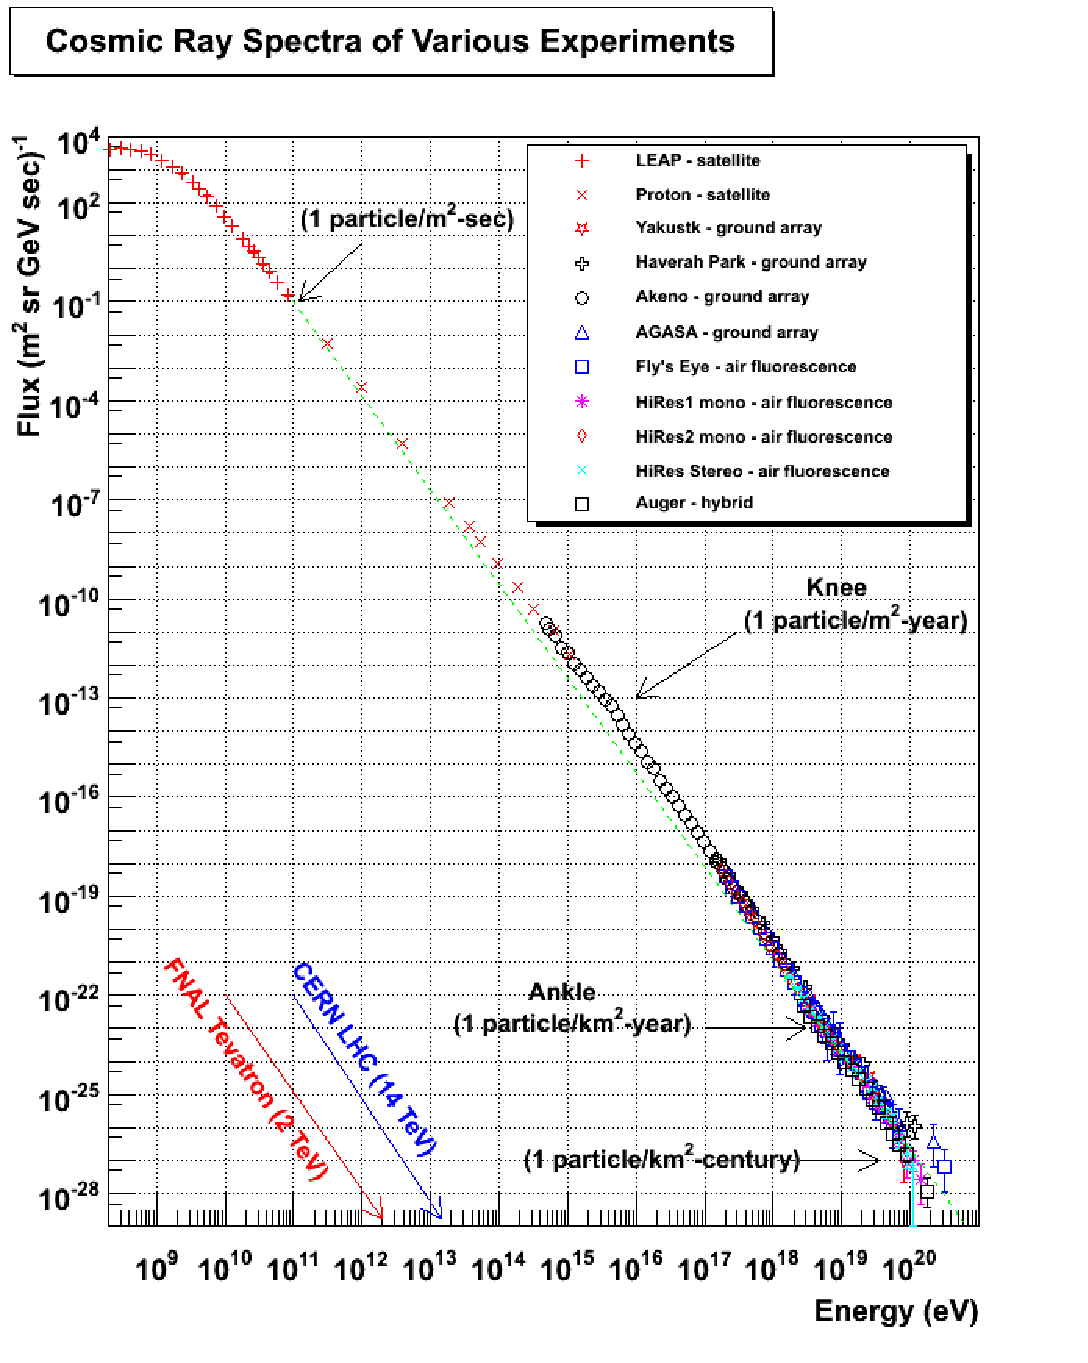
\includegraphics[width=0.77\textwidth]{./spectrum1.pdf}
        \caption{Cosmic ray spectrum from \cite{crspec} built with data from several experiments. Red and blue lines represent the energy spectrum covered by Tevatron and LHC accelerators. Green line shows the fit to a power law with spectral index 2.7.}
        \label{fig:CRspectrum}
    \end{figure}
    
    
    As already mentioned, it is possible to differentiate two \gls{cr} origins: galactic \gls{cr} and extragalactic \gls{cr}. Below the \textit{knee}, \glspl{cr} are produced in galactic accelerators (\glspl{snr}) and their maximum energy can be considered a limit on the acceleration that is possible to gain from these kind of objects. \glspl{cr} with energies above the \textit{ankle} are thought to come from extragalactic sources and so, their higher acceleration must come from different phenomena, more violent and energetic (\gls{agn}, \glspl{grb}, etc.). The Larmor radius defines the curved trajectory of charged particles moving perpendicular to a magnetic field. The "Hillas condition" \cite{1984hillascondition} sets a minimum requirement for the accelerators to reach certain energies, stating that a necessary condition to accelerate particles to ultrahigh energy is that of confinement, meaning that they can stay in the acceleration region as long as their Larmor radius is smaller than the size of the accelerator. For energies over the \textit{ankle} it starts to become larger than galactic scales, hence extragalactic \glspl{cr} propagate almost linearly and unaffected by the galactic magnetic field, while galactic (less energetic) \glspl{cr} propagate diffusively through the \gls{ism}. Figure \ref{fig:hillasdiag} shows the Hillas diagram, where different source classes are presented as function of their characteristic size and magnetic field strength.\\
The transition in the spectrum between galactic and extragalactic accelerators, although still not well understood, can be explained by the effect of the galactic magnetic field in the trajectories of \glspl{cr}, and the effect of galactic wind termination shocks as a re-acceleration process \cite{2016CRSpectrum}.\\


       \begin{figure}
        \centering
        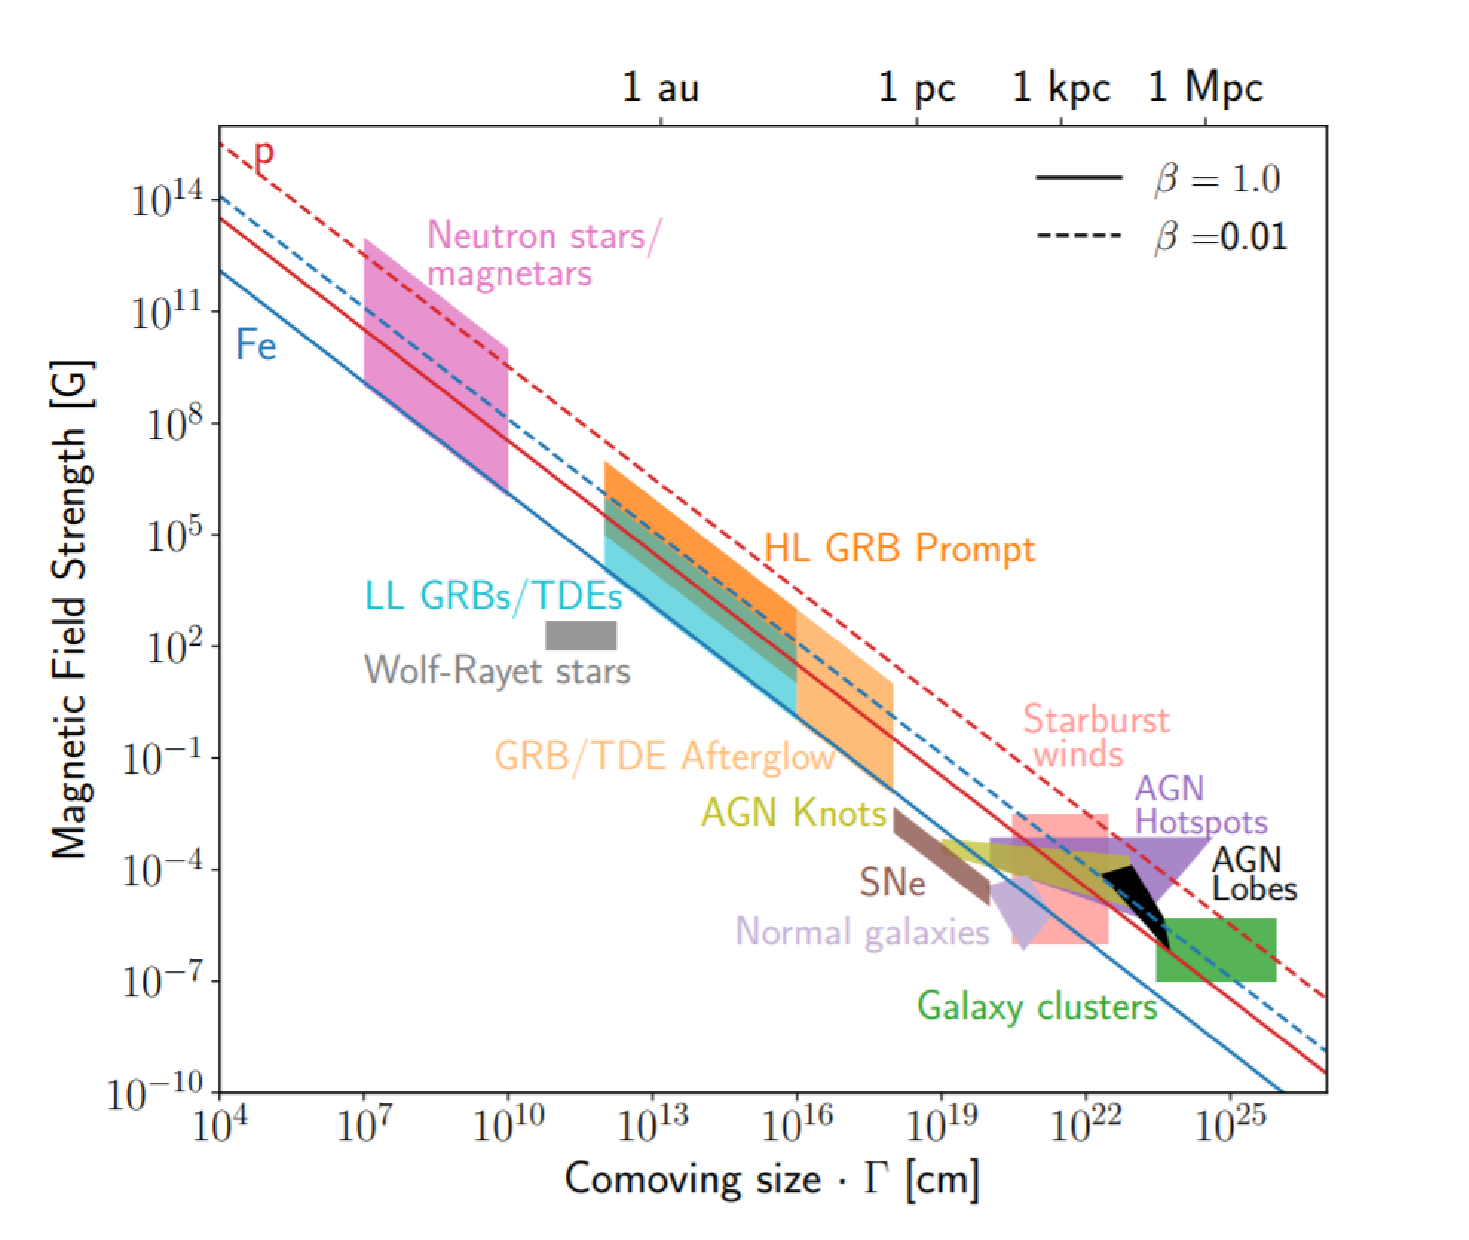
\includegraphics[width=0.77\textwidth]{Pictures/hillasdiagram.pdf}
        \caption{Hillas diagram, from \cite{2019openquestionsUHECR}. Source classes as a function of their characteristic radius $R$, given as the comoving size of the source times the Lorentx factor $\Gamma$, and the magnetic field $B$ in the comoving frame of the source. Solid (dashed) lines indicate the product of $B \times R$ beyond which confinement of protons (red) and iron (blue) nuclei with energy $10^{20}$ eV are possible for ouflows with velocity $\beta_{ish} = 1$($\beta_{ish} = 0.01$).}
        \label{fig:hillasdiag}
    \end{figure}
    
    The chemical composition of galactic \glspl{cr} is very similar to that of the Solar System (see figure \ref{fig:CRabundances}), suggesting a similar origin (stellar interiors) but with some discrepancies in certain elements. The most noticeable difference regards Li, Be and B, and to a lesser extent sub iron elements Mn, Cr, V, Ti and Se. The abundances of these elements are small in stars because they are rapidly consumed by nuclear reactions, but they are present in secondary \glspl{cr} due to \textit{spallation} of carbon and oxygen nuclei~\cite{particleastrophy} and other abundant heavy nuclei as Fe and Ni \cite{2018particleacceleration}.
    
    \begin{figure}
        \centering
        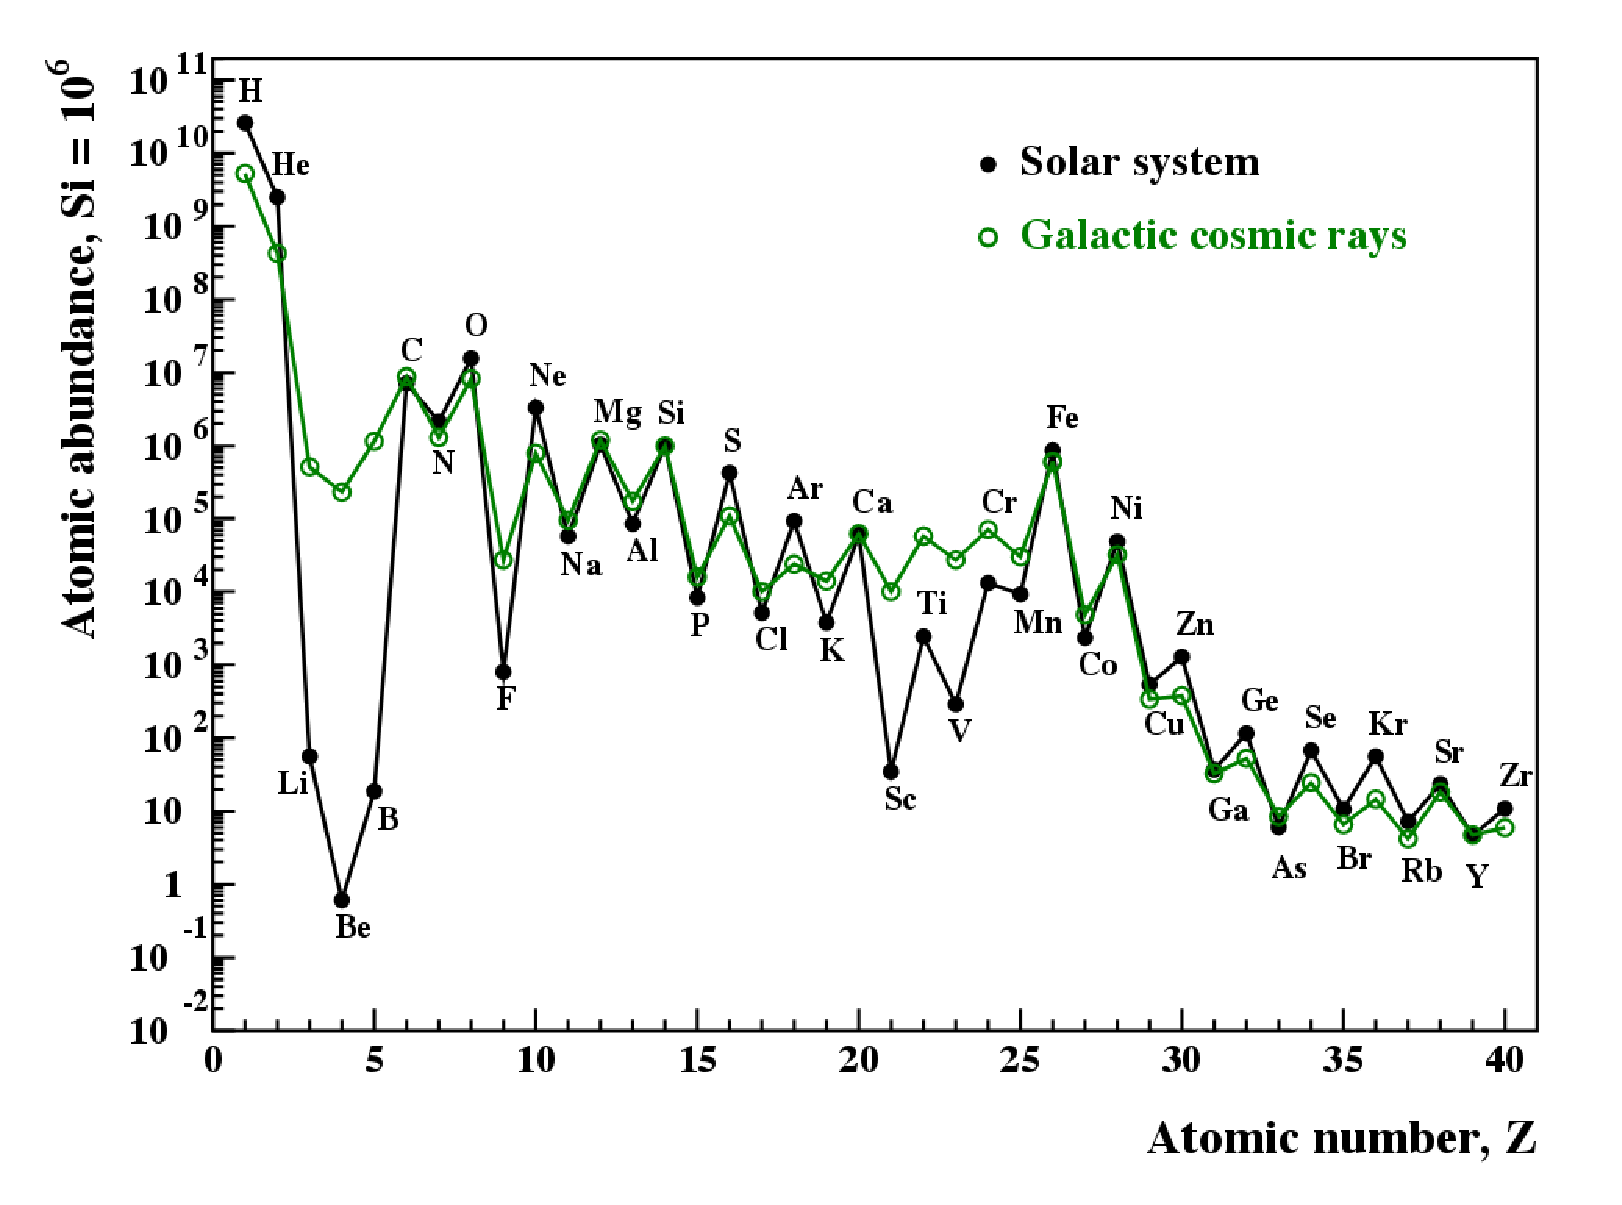
\includegraphics[width=0.77\textwidth]{Pictures/CRabundances.pdf}
        \caption{Abundances of elements of galactic \glspl{cr} compared to the Solar System, from \cite{2018particleacceleration}.}
        \label{fig:CRabundances}
    \end{figure}


\section{Acceleration mechanisms}\index{Acceleration}

Acceleration mechanisms take place in astrophysical plasmas which in general consists on thermal plasma components, a magnetic field and non-thermal distributions of fast particles. Within the plasma, turbulence and plasma waves take place, having an important role in particle acceleration.
The mechanisms that accelerate \glspl{cr} to the huge energies observed, that can reach up to $10^{20}$ eV are still a topic of debate and research in the high energy astrophysics field. Several particle acceleration mechanisms are proposed to explain the \gls{cr} spectrum, which should be able to achieve the highest energies measured for \gls{cr} and reproduce the spectral shape of a power law with an index $\sim 2.7$, and the abundances of elements measured \cite{Hillas:1985is}, \cite{2008particleaccelerationmech}, \cite{2009accelerationmech}.

\subsection{Electric field acceleration}

Electric fields parallel to magnetic fields can accelerate charged particles and can arise during magnetic field reconnection (the breaking and reconnecting of oppositely magnetic field lines in a plasma). Because ideal \gls{mhd} of plasmas require the paralell component of electric field to be null $E_{\parallel} = 0 $, non-ideal \gls{mhd} effects are needed to explain the development of $E_{\parallel} = 0$, such as resistivity or inertial effects on Alfvén waves (a type of \gls{mhd} wave where ions oscillate in response to a restoring force provided by an effective tension on the magnetic field lines)  \cite{2009accelerationmech}.\\
This kind of acceleration is believed to take place in magnetic reconnection of the Earth's magnetotail, accelerating auroral electrons; Also, reconnection in pulsar gaps (see section \ref{sec:pulsars}) could produce this kind of acceleration which should involve large oscillations in $E_{\parallel}$. 


\subsection{Stochastic acceleration}

Stochastic acceleration, also known as \textit{Second Order Fermi acceleration} or simply \textit{Fermi process}. This idea was developed by Enrico Fermi in 1949 \cite{Fermi:CRorigin} as a mechanism to explain acceleration of galactic \glspl{cr}. The basic concept is that particles can gain velocity after being reflected several times by randomly moving magnetized clouds in the \gls{ism}. Fermi showed that after a characteristic time $\tau_{esc}$, the spectrum of the accelerated particles would follow a power law. If the particle is moving with a pitch angle $\theta$ (the angle between the particle velocity vector and the local magnetic field), the gain in energy after a collision with a cloud moving with velocity $V$ will be \cite{highenergyastrophy}:

\begin{equation}
    \Delta E = E \left[ \frac{2Vcos\theta}{c^2}+2\left(\frac{V}{c}^2\right)\right]
\end{equation}

Where E is the energy of the particle before the collision. Between collisions the particle will be moving inside a plasma and will suffer scattering due to hydrodynamic waves, the total gain in energy has to be averaged over a set of random $\theta$ angles. The probability of a collision is proportional to the relative velocities of the particle (v) and the cloud ($V$). If $v \approx$ c the probability of a head-on collision $P \propto 1+(V/c)cos\theta$ is slightly higher than the probability of head-tail collision $P \propto 1-(V/c)cos\theta$ (see figure \ref{fig:fermiprocess}) hence the total, averaged in all $\theta$ angles between 0 and $\pi$, gain in energy will be positive:

\begin{equation}
    \left< \frac{\Delta E}{E}\right> = \frac{8}{3}\left( \frac{V}{c}\right)^2
\end{equation}

\begin{figure}
    \centering
    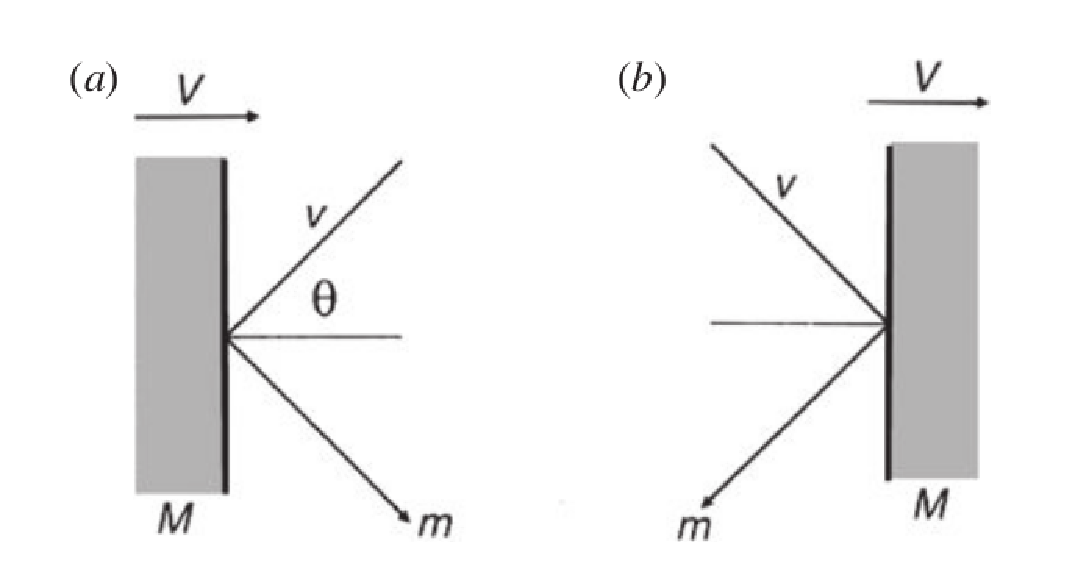
\includegraphics[width=0.77\textwidth]{Pictures/secondorderfermiacc.pdf}
    \caption{Collision of a particle of mass m with velocity v against a cloud of mass M and velocity V, a) head-on, b)head-tail, from \cite{highenergyastrophy}.}
    \label{fig:fermiprocess}
\end{figure}

Being the increase in energy \textit{second order} proportional to $V/c$. However, this process cannot be the main source of particle acceleration: the velocities of interstellar clouds in the \gls{ism} is too low ($V/c \simeq 10^{-4}$), the mean free path of \glspl{cr} in the \gls{ism} is too high (the number of collisions would be $\sim 1yr^{-1}$) and the particles should be injected in the acceleration region with already high velocities (\textit{injection problem} which actually is present in every acceleration mechanism).

\subsection{Diffusive Shock Acceleration}\index{diffshock}

The most popular acceleration mechanism in astrophysical plasmas, which is believed to take place in \glspl{snr} (the best candidates for galactic \gls{cr} production) is known as \gls{dsa} or \textit{First Order Fermi acceleration}. This mechanism revisits the original idea formulated by Fermi of particles colliding with randomly moving "magnetic mirrors" in the \gls{ism}, but  with all the collisions happening always head-on. For example, when two clouds are approaching each other and the particle bounces back and forth \cite{2009accelerationmech}. 
This process can happen in the presence of strong supersonic shock waves propagating through a diffuse medium, like the ones produced after a \gls{sn} explosion (see figure~\ref{fig:shock}). 
A flux of relativistic particles is assumed to exist in both sides of the shock, which are moving much faster than the latter. Each time a particle crosses to one side or the other, their velocity becomes isotropic in the frame of reference of the moving fluid. Since on every crossing the particle encounters gas moving towards it at a velocity proportional to the shock velocity (U), which for a fully ionized plasma composed by monoatomic perfect gas is $\sim 3/4 U$ (\cite{highenergyastrophy}) it will receive a boost in energy of the order $\sim U/c$. That is why this process is called \textit{first order} in counterpart to the classical second order Fermi acceleration where the energy gain in each collision is proportional to $\sim (U/c)^{2}$.  
\gls{dsa} is able to predict a spectral index of $\sim 2$, very close to the observed for galactic \gls{cr}. Also, is the only acceleration mechanism efficient enough to transfer the observed amount of energy in \gls{snr} to particles.
On the other hand, it exists an upper limit on the maximum energy that a particle can gain through \gls{dsa} which is set to $\sim 10^{14}$ eV \cite{1983maximumEinSNR}, so is still not enough to explain the full \gls{cr} spectrum, which reaches up to $\sim 10^{20}$ eV.
\begin{figure}
\centering
 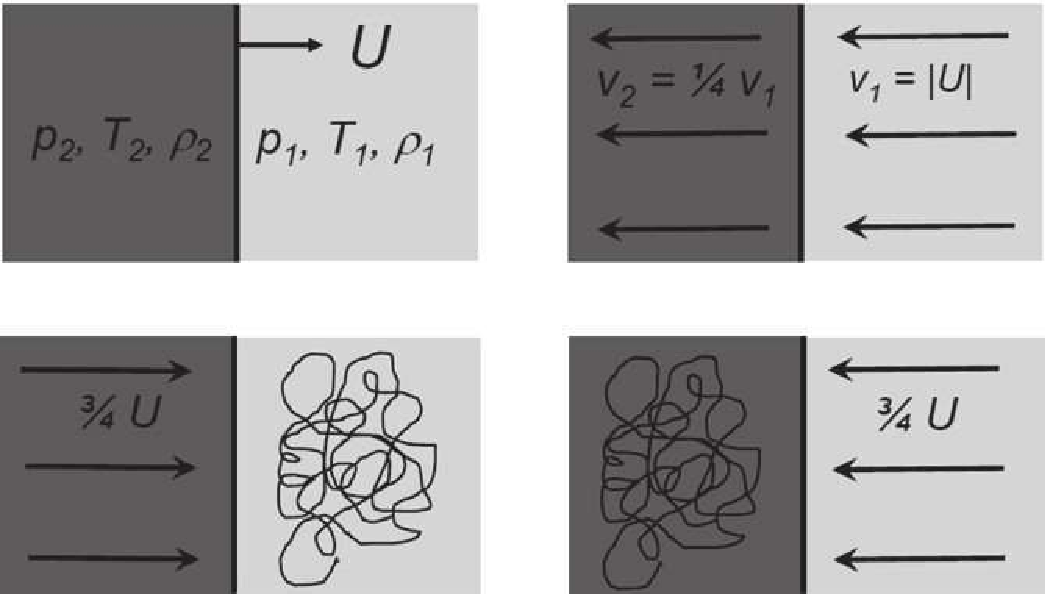
\includegraphics[width=0.77\textwidth]{./firstorderfermiacc.pdf}
  \caption{Scheme of the \textit{Diffuse shock acceleration} from \cite{highenergyastrophy}. \textit{Upper left}. Observer frame: A diffusive shock is propagating at velocity U. \textit{Upper right}. Frame where the shock front is at rest. The velocities of the gas in both sides of the front, assuming is fully ionized, have a ratio of 4. \textit{Lower left}. Frame of reference where the upstream gas is at rest, the distribution of velocities of the high energy particles is isotropic. \textit{Lower right} Same case as previous, but in the reference frame of the downstream gas.}
    \label{fig:shock}
\end{figure}

\section{Production of $\gamma$-rays}\index{Productionofgammas}\label{sec:gammaproduction}

Although \glspl{cr} have been known for many decades, it is difficult to make conclusions about their origin and acceleration mechanisms. As they are charged particles, their trajectories are deflected while travelling through the \gls{ism}, hence their incoming direction does not point towards the source of origin. Nevertheless, \glspl{cr} can interact with the medium producing $\gamma$-rays through several mechanisms, which reach the Earth undeflected, offering a way to indirectly study \gls{cr} origin, acceleration and diffusion in the \gls{ism}.  
When we talk about radiation production, we can distinguish between two main mechanisms which involve very different physical phenomena: thermal and non-thermal processes. A large fraction of the low energy radiation emitted by stars or interstellar dust is produced by thermal processes following a black body spectrum. To produce radiation as energetic as $\gamma$-rays a temperature of the order of $10^{10}$ K would be needed, which is something that was only reachable in the Big Bang conditions. Therefore, to understand the production of $\gamma$-rays we must study the so called \textit{non-thermal universe}, where radiation is produced by interactions of relativistic particles moving in electromagnetic fields.
In general, $\gamma$-rays are produced in two kinds of scenarios: leptonic emission (produced mainly by electrons) and hadronic emission (produced mainly by protons). Which one of those is dominant in astrophysical particle accelerators is still a subject of debate and will be commented in section \ref{sec:gammasources} about $\gamma$-ray sources.
In this section a brief summary on the different $\gamma$-ray production mechanisms (see figure \ref{fig:gammaproductionmec}) is given.

\subsection{Bremsstrahlung}\index{Bremss}

From the German 'braking radiation', the bremsstrahlung process occurs when a charged particle is decelerated by the electric field produced by an atomic nucleus. While their trajectory is deflected, the particle emits electromagnetic radiation with amplitude proportional to the magnitude of the deceleration suffered. The differential cross section for a particle of charge \textit{e}, mass \textit{m}, carrying an energy $E_{e}$ to radiate a photon between energies $E_{\gamma}$ and $E_{\gamma}+dE$ when interacting with the Coulomb field is:
\begin{equation} \label{eq:crosssectionbrems}
    \sigma(E_{e},E_{\gamma})dE_{\gamma} = 4\alpha Z^2r^{2}_{e}\frac{dE_{\gamma}}{E_{\gamma}}F(E_{e}, \nu)
\end{equation}

Where:
\begin{equation} \label{eq:fluxbremss}
    F(E_{e},\nu) = [1+(1-\nu)^2-\frac{2}{3}(1-\nu)]\left[ ln \left( \frac{2E_{e}}{m_{e}c^2} \frac{1-\nu}{\nu}\right)-\frac{1}{2}\right]
\end{equation}

Being $\alpha$ the fine structure constant and $\nu = E_{\gamma}/E_e$ the fractional energy carried by the photon \cite{1993MurthyGammaRay}. From equations \ref{eq:crosssectionbrems} and \ref{eq:fluxbremss} can be seen that the acceleration suffered by the particle is $\propto Ze^2/m$ , then while any charged particle can suffer bremsstrahlung, it is going to be much more efficient for electrons  than for protons which have a higher mass.
The photons emitted will have a continuum spectrum with energies of the same order of the particle, which for cosmic electrons in a gas is going to be a power law \cite{weekes2003HEAstrophy}. Bremsstrahlung is mainly efficient under high-density conditions. It takes place in gaseous nebulae that contain ionized gas, such as \gls{snr}, and in the intracluster medium of galaxy clusters \cite{MaozNushellAstro}. 

\begin{figure}
\begin{subfigure}{0.31\textwidth}
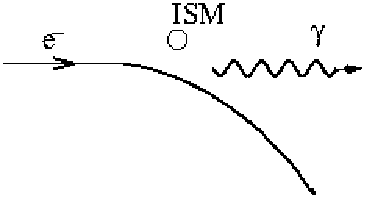
\includegraphics[width=\linewidth]{./bremsstrahlung.pdf}
\caption{Bremsstrahlung} \label{fig:1a}
\end{subfigure}
\hspace*{\fill} % separation between the subfigures
\begin{subfigure}{0.31\textwidth}
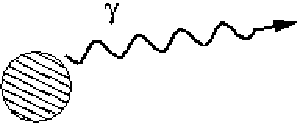
\includegraphics[width=\linewidth]{Pictures/thermalbrehms.pdf}
\caption{Thermal Bremsstrahlung} \label{fig:1b}
\end{subfigure}
\hspace*{\fill} % separation between the subfigures
\begin{subfigure}{0.31\textwidth}
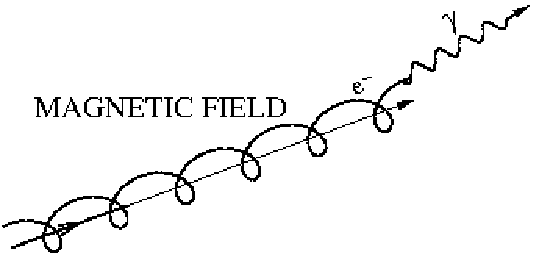
\includegraphics[width=\linewidth]{Pictures/synchrotron.pdf}
\caption{Synchrotron emission} \label{fig:1c} 
\end{subfigure} \\
\begin{subfigure}{0.31\textwidth}
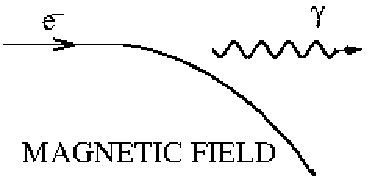
\includegraphics[width=\linewidth]{Pictures/curvaturerad.pdf}
\caption{Curvature radiation} \label{fig:1d}
\end{subfigure}
\hspace*{\fill} % separation between the subfigures
\begin{subfigure}{0.31\textwidth}
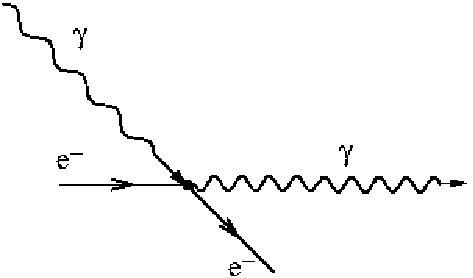
\includegraphics[width=\linewidth]{Pictures/IC.pdf}
\caption{Inverse Compton scattering} \label{fig:1e}
\end{subfigure}
\hspace*{\fill} % separation between the subfigures
\begin{subfigure}{0.31\textwidth}
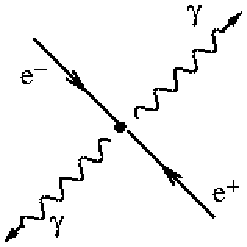
\includegraphics[width=\linewidth]{Pictures/electronpositron.pdf}
\caption{Electron-positron annihilation} \label{fig:1f} 
\end{subfigure}
\\
\begin{subfigure}{0.31\textwidth}
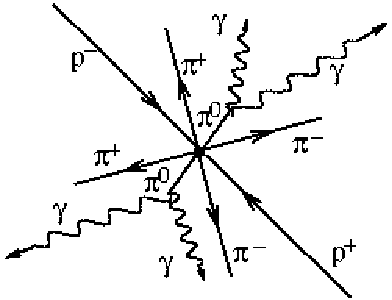
\includegraphics[width=\linewidth]{Pictures/protonantiproton.pdf}
\caption{Proton-antiproton annihilation} \label{fig:1g}
\end{subfigure}
\hspace*{\fill} % separation between the subfigures
\begin{subfigure}{0.31\textwidth}
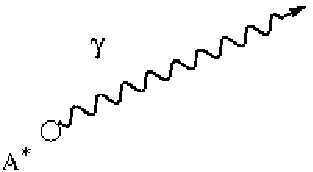
\includegraphics[width=\linewidth]{Pictures/radioactiveemission.pdf}
\caption{Radioactive emission} \label{fig:1h}
\end{subfigure}
\hspace*{\fill} % separation between the subfigures
\begin{subfigure}{0.31\textwidth}
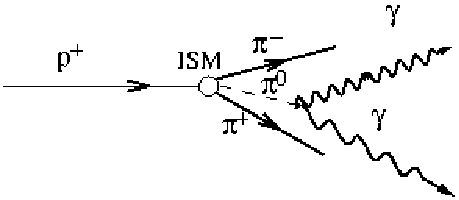
\includegraphics[width=\linewidth]{Pictures/hadrocollision.pdf}
\caption{Hadronic collision} \label{fig:1i} 
\end{subfigure}
\caption{Diagrams of the different $\gamma$-ray production processes. Figures extracted from \cite{OyaVallejo:2010ipa} \label{fig:gammaproductionmec}.}
\end{figure}

\subsection{Inverse Compton scattering}\index{inversecompton}\label{sec:IC}

\gls{ic} scattering is the inelastic interaction where a relativistic charged particle transfer a considerable amount of energy to a photon. In the frame of reference of the electron the photon will suffer an "energy boosting" \cite{weekes2003HEAstrophy}. The energy of the scattered particle is $E = \Gamma m c^2$, where $\Gamma$ is the Lorentz factor, and we can define the parameter $\alpha = h\nu/mc^2$, where $\epsilon = h\nu$ is the initial energy of the photon. We can differentiate between two regimes depending on the initial energy of the photon:

\begin{itemize}
    \item \textit{Thomson regime}: For low values of $\alpha$, particle recoil can be neglected and the energy of the photon after the scattering follows:\\
    \begin{equation}
         E_{\gamma}  \simeq \frac{4}{3}\epsilon \gamma^{2}
    \end{equation}
    
    \item \textit{Klein-Nishina regime}: For large values of $\alpha$, particle recoil is significant and in this case the energy of the photon after the interaction is:
    \begin{equation}
        E_{\gamma}  \simeq \frac{1}{2} E
    \end{equation}
\end{itemize}

Photons from the \gls{cmb} are typical targets for \gls{ic} scattering, together with synchrotron photons or photons thermally emitted by astrophysical sources. This mechanism is predominant in \gls{vhe} $\gamma$-ray emitters, like in the jets of \gls{agn} and TeV blazars. 
The spectrum of the photons boosted by this process will follow a power law related to that of the population of relativistic electrons in the medium ($\propto E_e^{-\Gamma_e}$ ):

\begin{equation}
    \frac{dN_{\gamma}}{dE} \propto E^{\frac{-(\Gamma_e + 1)}{2}}
\end{equation}


\subsection{Synchrotron emission}\index{Synchro}

Synchrotron emission is produced when a charged particle is moving in a magnetic field. The particle will follow an spiral path, with constant velocity along the field lines, while being accelerated towards the center of its orbit. The particle will suffer energy losses that for relativistic particles follow a continuum spectrum \cite{weekes2003HEAstrophy} with a critical frequency $w_c$ at which the maximum power is emitted:

\begin{equation}\label{eq:maxwsynchro}
    w_c = \frac{3}{2}\frac{eB}{mc}\Gamma^2\,sin\phi
\end{equation}

Where $e$ and $m$ are the charge and mass of the particle, $B$ is the magnetic field, $\Gamma$ is the Lorentz factor and $\phi$ kis the pitch angle bewteen the direction of the magnetic field and the particle.
The total energy loss is given by
\begin{equation} \label{eq:powersynchro}
    -\frac{1}{c}\left( \frac{dE}{dt} \right) = \frac{2e^4}{3m^2c^4}\Gamma^2 B^2  erg \, cm^{-1}
\end{equation}

Following \ref{eq:powersynchro} the power emitted is inversely proportional to the mass of the particle so it will be comparatively much more efficient for electrons than for protons. 

Synchrotron radiation of ultra-relativistic particles is the most important contribution to the non-thermal universe (radio, X-rays...). According to \ref{eq:maxwsynchro} the production of \gls{he} $\gamma-rays$ will require too high values of B and $E_e$, but regions emitting synchrotron radiation contain relativistic electrons capable of \gls{ic} scattering \cite{HarwitAstroconcepts},  which will acquire much higher energies. 

\subsection{Curvature radiation}

In presence of very strong magnetic fields, of the order of $10^{11}$-$10^{13}$ G, electron and positrons will be forced to follow a trajectory parallel to the magnetic field lines. Since the lines are curved, with a curvature radius $\rho_{c}$, the particle will emit \textit{curvature radiation} in the direction of movement, with a characteristic photon energy \cite{Pulsars}:
\begin{equation}
    E_{c} = \frac{3}{2} \Gamma^3\frac{\hbar c}{\rho_c}
\end{equation}

Typical environment where curvature radiation takes place are the surroundings of pulsars, due to the extremely high magnetic fields close to their surfaces. An electron with an energy of 10 TeV moving along a field line with a curvature of $10^8$ cm, which is typical for pulsars, emits photons of energy $\approx 2.5$ GeV \cite{1993MurthyGammaRay}. 



\subsection{Matter-Antimatter annihilation}\index{electronpositron}

Matter-antimatter pair annihilation processes can produce $\gamma$-rays. The most common case is electron-positron annihilation ($e^-e^+\rightarrow 2\gamma$). If the two particles are at rest, they produce $\gamma$-rays with energy equal to their masses (0.511 MeV). If the particles are thermalized but with low energies, such as the electrons of the ambient gas/plasma, they form the unstable state called positronium which can annihilate into 3 photons forming a continuum \cite{2004VHECosmicGammaRadiation}.
For relativistic particles interacting in-flight, the annihilation cross section is:

\begin{equation}\label{eq:eeannihilation}
    \sigma_{A} = \frac{\pi r_{e}^{2}}{\Gamma} [ln(2\Gamma)-1]
\end{equation}

Where $\Gamma=E_e/m_ec^2$ is the Lorentz factor of the positrons and $r_e=e^2/m_ec^2 = 2.82 \times 10^{-13} $cm is the classical radius of the electron. The result of the interaction is the emission of two photons with a continuum of energies. At very high energies, the cross section of equation \ref{eq:eeannihilation} is quite low, leading to very high mean free paths and long lifetimes for the positrons, which typically will be affected by other processes before annihilating. Positrons can lose energy gradually without escaping the galaxy until the cross section is high enough and they annihilate \cite{1993MurthyGammaRay}.

Proton-antiproton annihilation can also produce $\gamma$-rays indirectly by the production of neutral pions $\pi^0$ which decay into $\gamma$-rays later on \cite{1967protonantiproton}. In theory, antiprotons can be produced by interactions of protons with matter, but this process is much less efficient than the direct production of $\pi_0$ mesons \cite{weekes2003HEAstrophy} so the production of $\gamma$-rays this way is considered marginal. 

\subsection{Hadronic collisions}

While most of the processes described above were dominated by electron interactions (leptonic scenario), we now focus on the processes that constitute the hadronic contribution to the production of $\gamma$-rays, which are believed to be the dominant $\gamma$-ray production processes in \glspl{snr} and \gls{agn}. 

Protons accelerated to relativistic energies in extreme environments, such as strong magnetic fields or jets can collide with other hadrons producing mesons, kaons and hyperions. The most common interaction is the proton-proton collision to produce pions ($\pi$ mesons):
\begin{equation}
    pp \rightarrow pp \pi^{0}
\end{equation}
With a threshold energy of the proton, which is the minimum kinetic energy the pair of protons must have in the collision to produce the meson:
\begin{equation}
    E_{p} = 2m_{\pi^{0}}c^{2}\left(1+\frac{m_{\pi^{0}}}{4m_{p}} \right) \simeq 280 MeV
\end{equation}

Where $m_{\pi^{0}}$= 134.97 MeV is the mass of the $\pi_{0}$-meson and $m_p$=938.27 MeV is the mass of the proton \cite{2004VHECosmicGammaRadiation}. 

Neutral pions $\pi^{0}$ decay into $\gamma$-rays within a short lifetime $\tau = 8.6 \cdot 10^{-17}$s through the channels:
\begin{equation}
    \pi^{0} \rightarrow \gamma\gamma 
    \\ \hspace{3cm}(98.8 \%)
\end{equation}
\begin{equation}
    \pi^{0} \rightarrow e^{-}e^{+}\gamma 
    \\ {}\hspace{3cm}(1.2 \%)
\end{equation}

Then the energy of the photons emitted by the $\pi^{0}$ peaks at $E_{\gamma} = m_{\pi^{0}}c^{2}/2 \simeq = 67.5$ MeV, but in the laboratory frame of reference this energy depends on the energy of the $\pi^{0}$ and the angle of the proton trajectory with respect to the $\pi^{0}$ allowing the emitted $\gamma$-rays to reach very high energies.

The collision of protons can also produce charged mesons, which can decay into neutrinos $\nu_{e,\mu}$ with an spectrum similar to that of the photons \cite{2004VHECosmicGammaRadiation}. Finding a correlation between $gamma$-ray emission and astrophysical neutrinos from a certain source would be an unequivocal way to differentiate between leptonic and hadronic emission. Their spectrum shape and the lack of correlation with X-rays could be other ways to distinguish hadronic and leptonic emission. 


\section{$\gamma$-ray Absorption mechanisms} \label{sec:absorption}
 
Because $\gamma$-rays are very energetic, they can travel long distances without being altered. However there are mechanisms that can produce losses of energy of astrophysical $\gamma$-rays or their total absorption, altering the spectrum of that is detected from Earth. These mechanisms can be divided in $\gamma$-matter interactions and $\gamma-\gamma$ processes.

\subsection{Interaction with electrons: Compton effect}

Compton effect is produced when a photon is scattered by an electron, shifting the wavelength of the photon to lower energies. The shift in the wavelength goes like:

\begin{equation}
    \lambda '-\lambda = \frac{h}{m_e c}(1-cos\theta)    
\end{equation}

Where $\lambda'$ is the wavelength of the scattered photon, $\lambda$ the wavelength of the incident photon and $\theta$ is the scattering angle. In the standard \gls{ism} density of 1 atom cm$^-3$, for distances of $\sim$ 10 kpc, the mean free path for photons of 1 MeV would be of 2 Mpc, thus the Compton effect is negligible. In hot dense plasmas however, were densities are much higher, the effect can be quite important \cite{1993MurthyGammaRay}.

This effect is used in Compton $\gamma$-ray telescopes such as described in section \ref{sec:comptondetectors}. 

\subsection{Pair production processes}

Pair production is the opposite process to pair annihilation, where two photons interact to produce a pair $e^{-}e^{+}$. This is the most common absorption mechanism for \gls{he} and \gls{vhe} photons.
A $\gamma$-ray with energy $\epsilon_1$ which collides with a target photon with energy $\epsilon_2$ will produce a pair of particles of mass $m$ is $\epsilon_1$ is greater than a threshold energy:

\begin{equation}
    \epsilon_t = \frac{2m^2c^4}{\epsilon_2(1-cos\theta)}
\end{equation}

where $\theta$ is the angle between the trajectories of the photons. In astrophysics, this process occurs when energetic photons traveling through the Universe encounter a radiation field, such as the \gls{cmb} ($\epsilon_t \approx 4\times10^{14}$eV) or the light of stars ($\epsilon_t \approx 4\times10^{11}$). Even though photon-photon collisions are not generally frequent, because the spatial density of the target photons is not very large ($\approx 400$ cm$^{-3}$ for the \gls{cmb} radiation n and $\approx 5\times10^{-3}$cm$^-3$ for extragalactic starlight) the attenuation effect can be appreciated, specially for \gls{vhe} photons coming from high redshifts. 
This process also occurs when $\gamma$-rays penetrate the atmosphere and are absorbed, leading to the production of \gls{eas}, which are the key for ground based $\gamma$-ray detectors and will be explained in section \ref{sec:eas}.


\subsection{The Extragalactic Background Light}

The \gls{ebl} is the accumulated radiation in the universe due to star formation processes and the emission from \glspl{agn}. It is a fundamental constituent of the universe that permeates it uniformly. The direct measurement of the \gls{ebl} are very difficult task, mainly because of the foreground light from the Solar System.  Phenomenological approaches try to predict an \gls{ebl} model based on galaxy formation and evolution during the history of the universe and several direct measurements have been done from the far infrared to the optical to set constrains on the density and spectrum of the \gls{ebl} \cite{DominguezEBL}. Besides the different proposed models, it is accepted that the energy density is characterized by two peaks, as seen in figure \ref{fig:eblmodel}. The first peak, found at $\sim 1\mu$m is the stellar component and the second peak at $\sim 100 \mu $m is the dust component, the light re-emitted by cosmic dust. 

\begin{figure}
\centering
 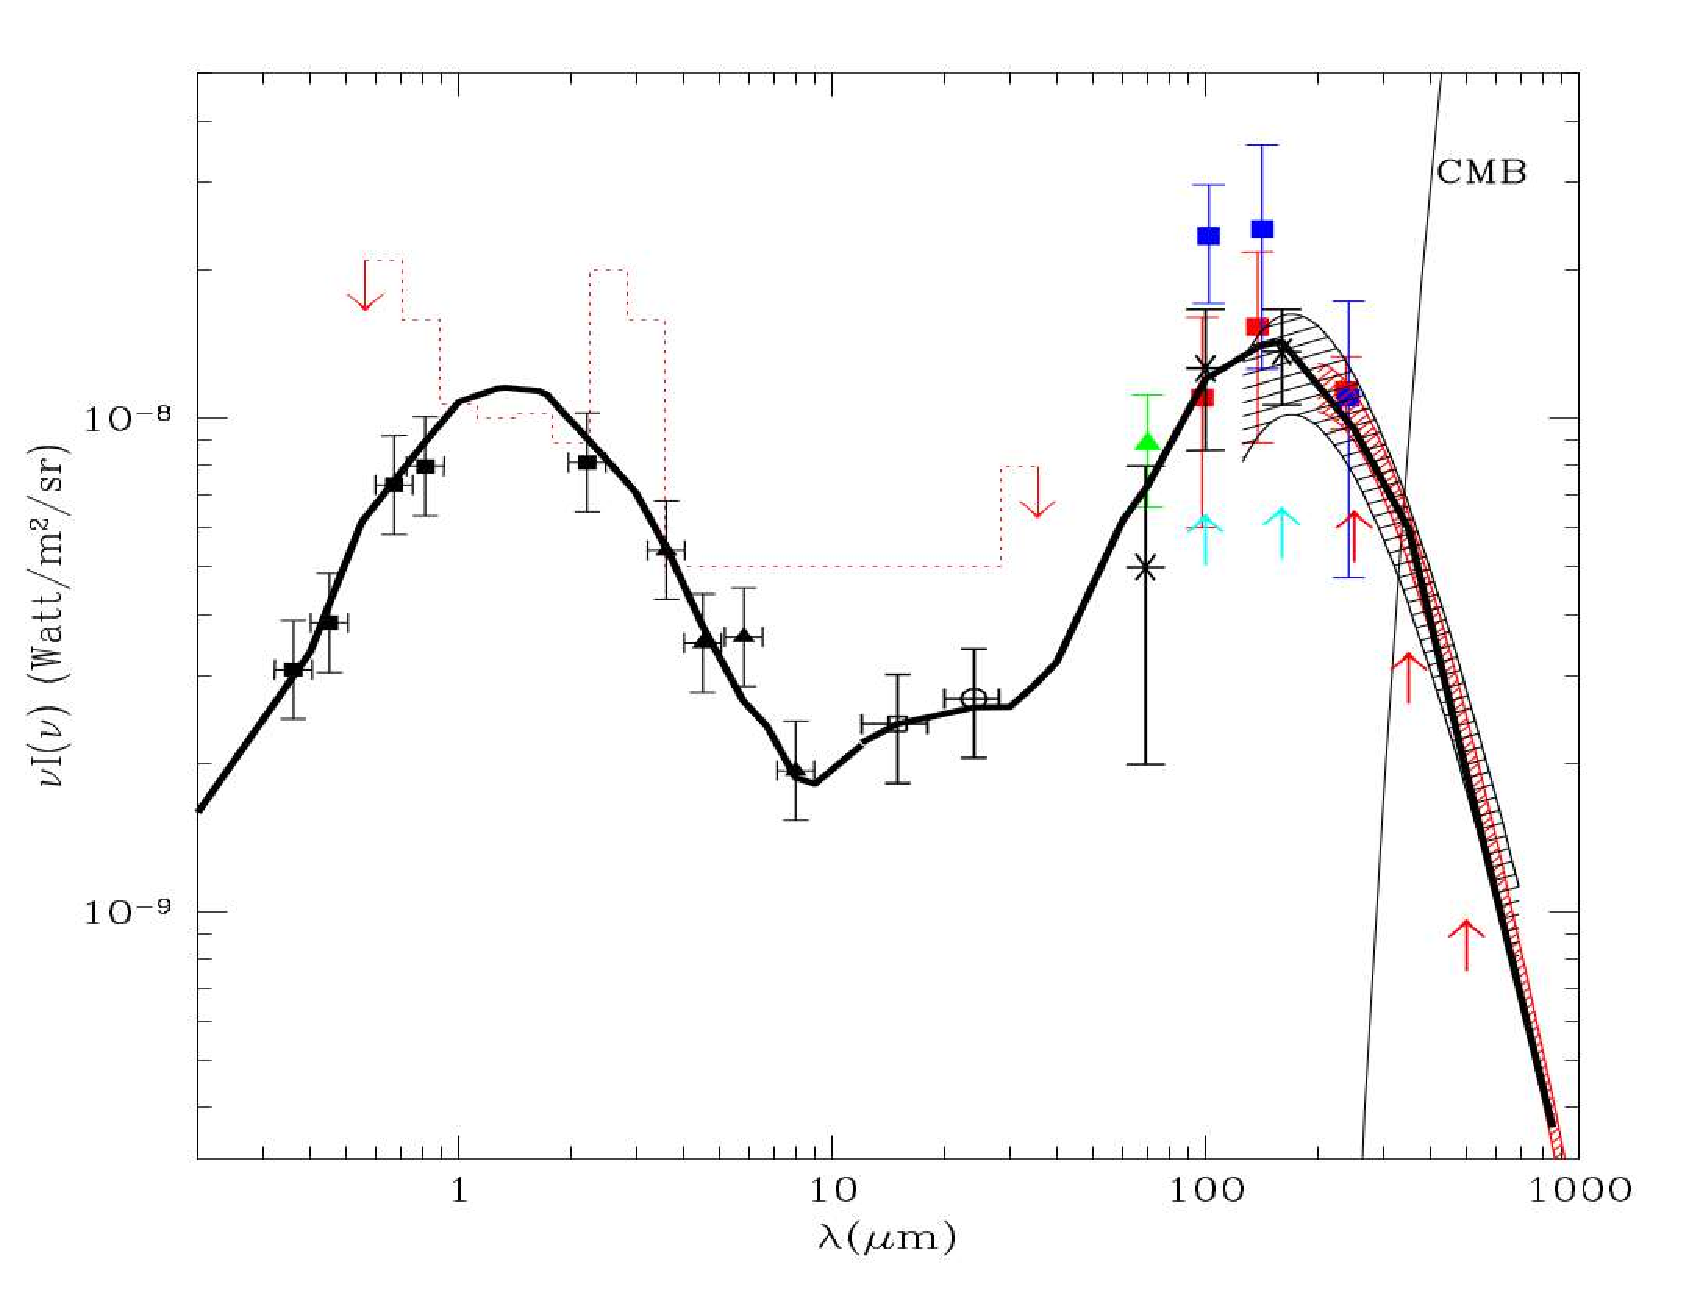
\includegraphics[width=0.77\textwidth]{./eblmodel.pdf}
  \caption{Best fit model prediction of the \gls{ebl} energy density from \cite{FranceschiniEBL} (thick black line).}
    \label{fig:eblmodel}
\end{figure}

\gls{ebl} photons are a typical target for $\gamma$-rays to produce pair production. The attenuation to the spectrum of a $\gamma$-ray source at the energy $E$ follows the form:

\begin{equation}
    F = F_{0}(E) e^{\tau(E,z)} 
\end{equation}

Where $F$ is the observed flux and $F_{0}$ the intrinsic spectrum of the $\gamma$-ray source, $\tau$ is the optical depth which depends on the energy and the redshift $z$ (as shown in figure \ref{fig:depth}). As a consequence of this dependence, for each energy there is a distance (redshift) at which the universe is optically thick to $\gamma$-rays, when the optical depth is equal to 1. The spectrum of the $\gamma$-ray source will suffer a cutoff at the energy that reaches the threshold optical depth, which decreases rapidly with redshift. Observations of this effect in distant sources in the \gls{vhe} range is very useful to characterize the EBL in an indirect way, comparing the expected spectrum to the measured one \cite{2017ICRCEBL}.

\begin{figure}
\centering
 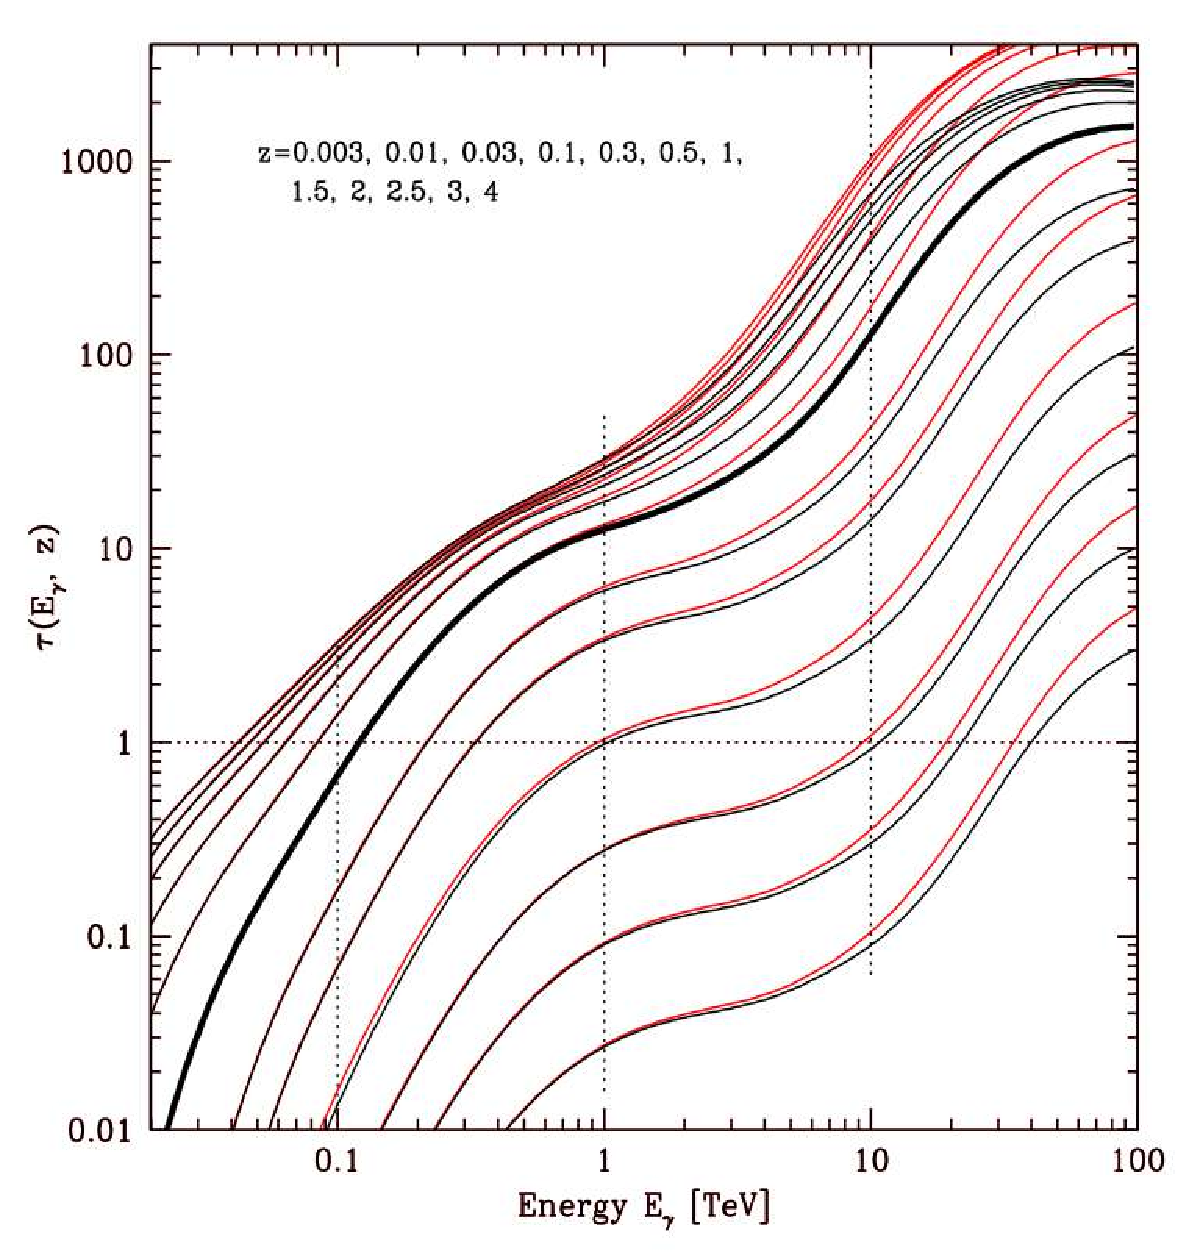
\includegraphics[width=0.77\textwidth]{./opticaldeph.pdf}
  \caption{Optical depth due to photon-photon collision as a function of energy for different redshift values, from \cite{FranceschiniEBL}.}
    \label{fig:depth}
\end{figure}


\section{Dark Matter and $\gamma$-rays: WIMP annihilation} \label{sec:DM}

The nature of \gls{dm} is one of the most important open questions in modern physics. There are many probes that suggest that the universe is composed of something more than the visible matter: From the Fritz Zwicky measurements on the velocity dispersion in the Coma galaxy cluster \cite{Zwicky} and the rotation curves of high-luminosity spiral galaxies obtained by Vera Rubin \cite{1978Rubin}, to the much more modern measurements of the \gls{cmb} by Planck \cite{2014Planck}, all of them point to the existence of a non-baryonic type of matter which only interacts gravitationally with \gls{sm} particles. Cosmological simulations and cosmological probes such as \gls{wmap} point to a hierarchical structure formation of the universe, where small structures formed first and then merged to the larger. To accomplish for that model, if \gls{dm} is formed by particles, they should be non-relativistic (Cold dark matter) which decoupled from the thermal equilibrium in the early universe. Hot dark matter models, where \gls{dm} particles would be still largely relativistic (like neutrinos), would lead to large structures forming first and fragment out later \cite{2003Olive}. 

With these assumptions, we can derive the number density evolution of \gls{dm} particles today. In the early universe, \gls{dm} and \gls{sm} particles were in thermal equilibrium with the photon bath emitted in the Big Bang, and reactions of annihilation and formation of particles were taking place at the same rate. While the universe expanded, these reactions started to be slower than the rate of expansion, so these particles \textit{decoupled} from the thermal bath. This is the moment of \textit{freeze-out}, before that particles had an equilibrium number density $Y_{eq}$, which evolves with time while the universe keep expanding. For \gls{dm} and using the Boltzmann equation, the number density evolution $dY/dx$ follow the equation:

\begin{equation}
    \frac{dY}{dx} = -\frac{xs\langle\sigma v\rangle}{H(m)}(Y^{2}-Y^{2}_{eq})
    \label{eq:dmabundance}
\end{equation}

Where m is the mass of the \gls{dm} particle, x is the scaled time variable $x=m/T$ being T the temperature of the photon bath at the moment of freeze out, s is the total entropy density of the universe, Y is actually defined as the number density of \gls{dm} rescaled to s ($Y = n/s$) to account for the expansion of the universe, $\langle\sigma v\rangle$ is the velocity averaged cross section for the reaction of \gls{dm} particles annihilating into \gls{sm} particles and H(m) is the Hubble rate (which defines the rate of expansion of the Universe) defined as $H(x) = H(m)/x^2$.\\
While the annihilation rate of the particles is higher than the expansion rate of the universe ($\Gamma \gg H $), the number density $Y$ remains close to $Y_{eq}$. After the moment of freeze-out $x_f$ ($\Gamma \ll H$), the number density will remain almost constant as shown in figure \ref{fig:DMn}. 

\begin{figure}
\centering
 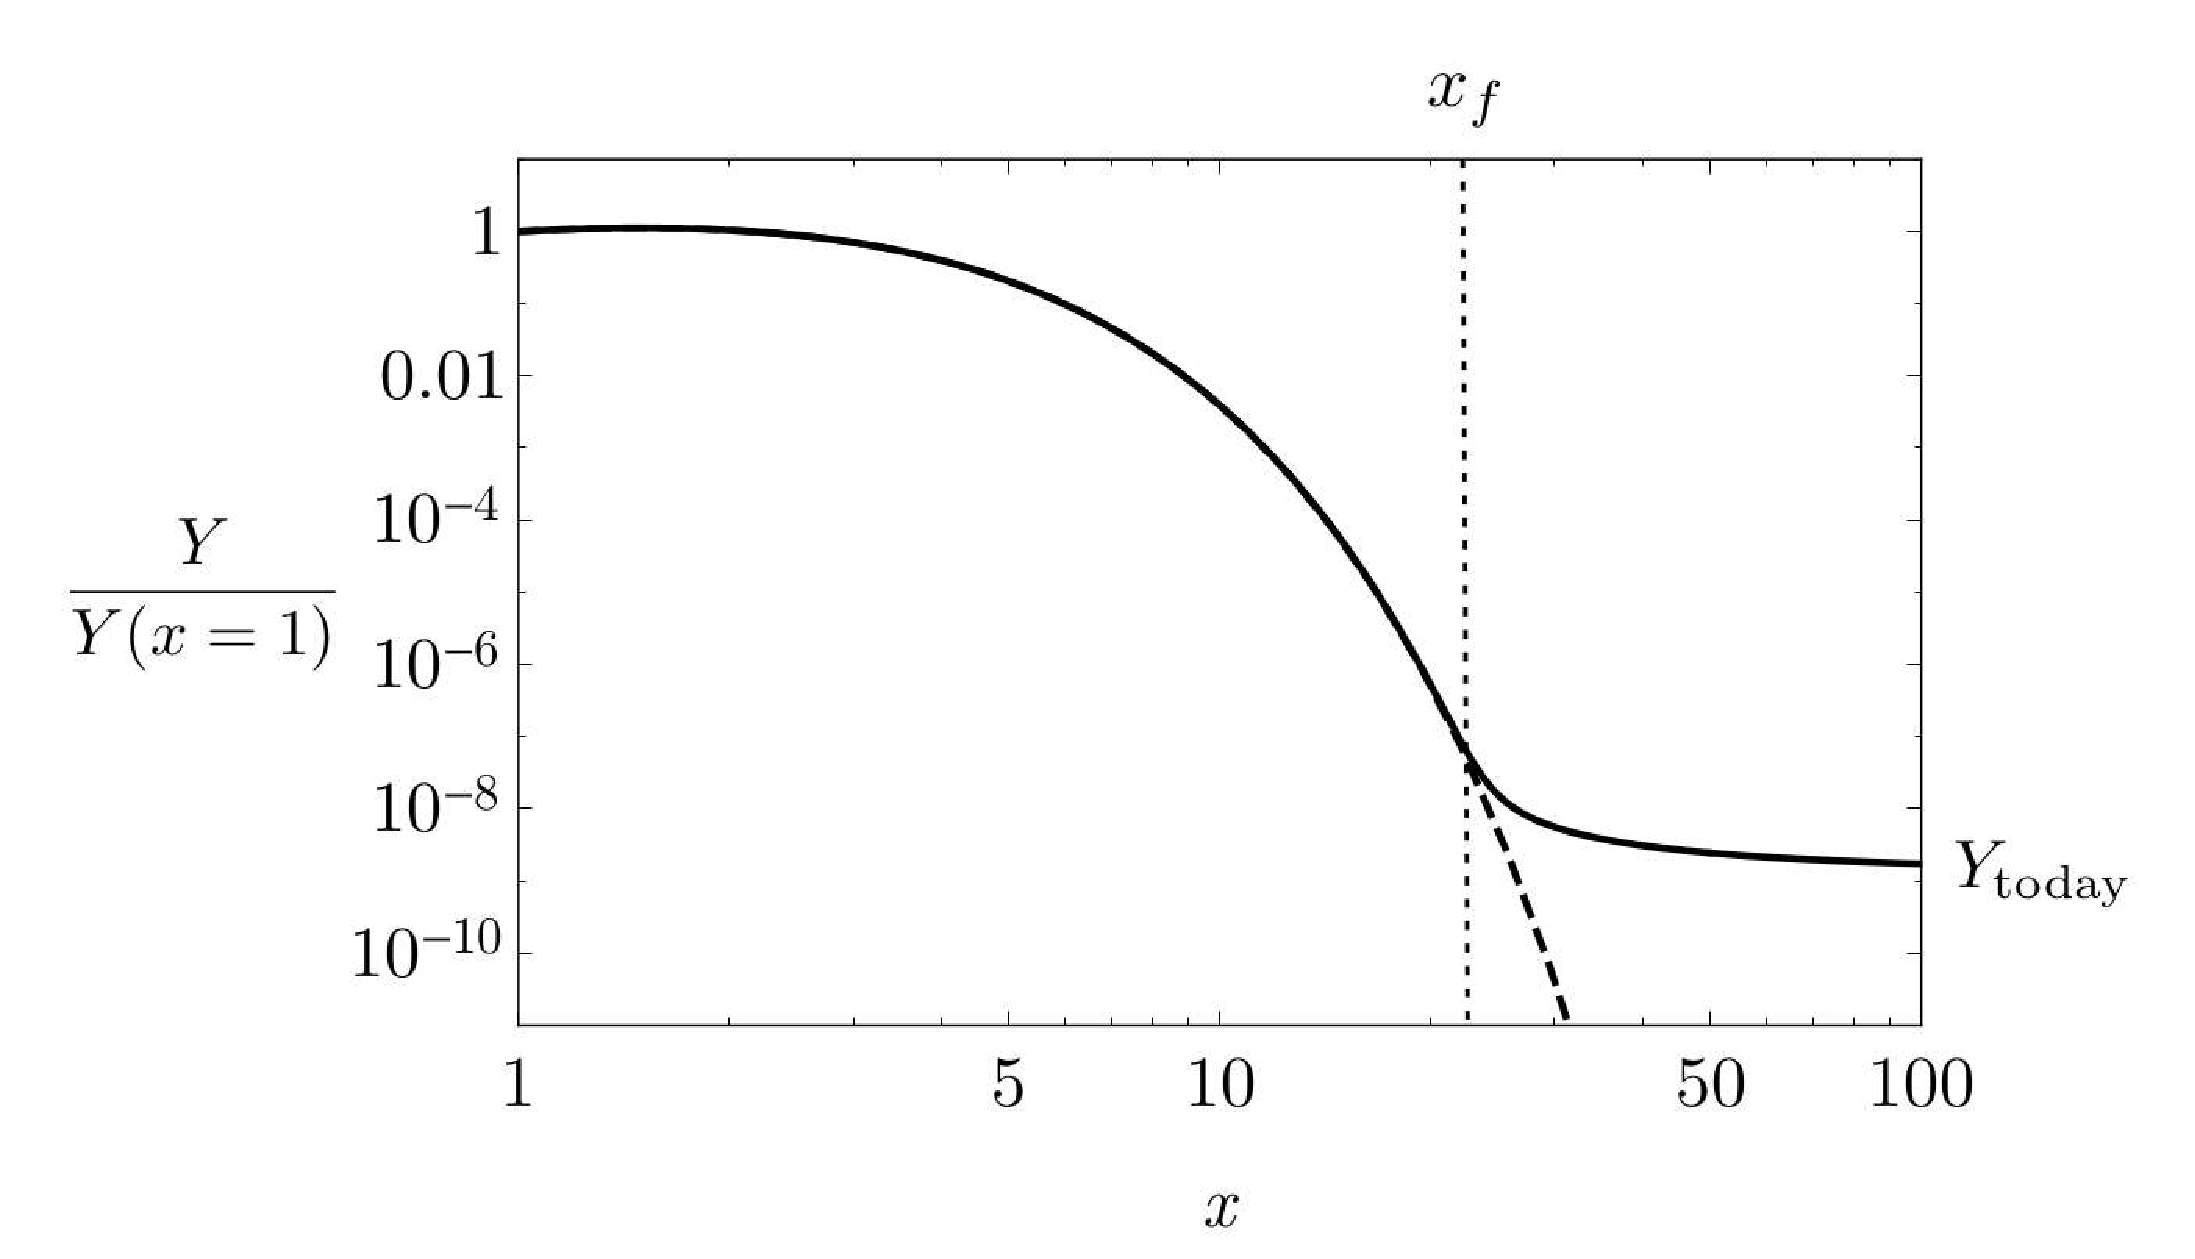
\includegraphics[width=0.77\textwidth]{./DMnumberdensity.pdf}
  \caption{Evolution of Cold Dark Matter number density with time variable $x$, $x_{f}$ is the time of \textit{freeze-out}, from \cite{2017DMlectures}.}
    \label{fig:DMn}
\end{figure}

Following the approach of \cite{2017DMlectures}, after freeze-out, the evolution of \gls{dm} abundance can be written as:

\begin{equation}
    \frac{dY}{dx}\approx - \frac{\lambda}{x^{n+2}} \textrm{, where } \lambda = \frac{\langle\sigma v \rangle_{0}s_{0}}{H(m)}
\end{equation}

To define $\lambda$ the dependency of the cross section and entropy with $x$ was pulled out through the change of variables: $\langle\sigma v \rangle = \langle\sigma v \rangle_{0} x^{-n}$ and $s=s_{0}x^{-3}$, where n is an exponent which depends on details of the particle physics model. Taking n=0, the \gls{dm} abundance today would be $\simeq x_{f}/\lambda$.
There is no \gls{sm} particle which can explain the cosmic density of \gls{dm} measured today $\Omega_{\chi}$, but if we consider a weak interacting particle in the weak mass regime ($m_{\chi}\sim 100$ GeV), the correct \gls{dm} density measured by Planck and \gls{wmap} arises naturally:

\begin{equation}
    \Omega_{\chi}=\frac{m_{\chi}s_{today}Y_{today}}{\rho_{cr}}\rightarrow \Omega_{\chi} h^{2}\sim \frac{10^{-26}cm^{3}/s}{\langle\sigma v\rangle} \simeq 0.1 \left(\frac{0.01}{\alpha}\right)^{2}\left( \frac{m_{\chi}}{100 GeV}\right) 
\end{equation}
where $\rho_{cr}$ is the critical density in the universe required for it to be at balance.
This is called the "WIMP miracle" for the theoretical \glspl{wimp} which have some candidates within the \gls{susy} theory. Although the annihilation of these particles would be strongly suppressed after freeze-out, it can still occur in regions with high \gls{dm} density. The products of this annihilation are pairs of \gls{sm} particles that can be detected as an excess signal in particle detectors, giving an indirect evidence of the presence of \gls{dm}.\\
 $\Gamma$-ray astrophysics contribute this way to the indirect detection of \gls{dm} signatures: Two \gls{dm} particles can annihilate directly into a pair of $\gamma$-rays with a characteristic line spectrum with $E_{\gamma}=m_\chi$ or they can annihilate into pairs of other \gls{sm} particles which afterwards decay giving out a continuum spectrum of $\gamma$-rays.\\
The differential flux of photons produced by \gls{dm} annihilation is described as:

\begin{equation}
    \frac{d \Phi}{dE}=\frac{1}{8 \pi} \frac{<\sigma v>}{m_{\chi}^2} \frac{d N_{\gamma}}{dE} \int_{\Delta\Omega}\int_{l.o.s} dl \rho^2(\vec{l})
\label{eq:flux}
\end{equation}
Where $dN/dE$ is the spectrum of $\gamma$-rays from annihilation of a pair of dark matter particles, $\langle\sigma v\rangle$ is the thermal velocity averaged annihilation cross section, $m_\chi$ is the \gls{dm} particle mass and $\rho$ is the dark matter density profile. If \gls{dm} particle is not its own antiparticle, equation \ref{eq:flux} should be multiplied by a factor 1/2. \\
The first term of the equation comes from the already discussed particle physics, depends on the annihilation channel and the mass of the particle. The integral second term is known as the J-factor and is the integral over the line of sight and solid angle $\Delta\Omega$ of the squared \gls{dm} density profile ($\rho$) and it is dependent on the source. The most simple density profile for a dark matter halo that we can think of is a self-gravitating isothermal gas sphere, where:

\begin{equation}
    \rho(r) \propto 1/r^2
\end{equation}

However, to address the actual physics of galaxies evolution, we need to relay on structure formation simulations which follow the initial \gls{dm} density perturbations until the formation of current halos. From these simulations and from actual observations \cite{1998Krav} we know that the \gls{dm} density profile can be well reproduced as a six-parameters function of distance \textit{r} from the center of the profile \cite{1990Hern}\cite{1996Zhao}\cite{1998Krav}:

\begin{equation}
    \rho(r) = \frac{\rho_{0}}{\left(\frac{r}{r_{S}}\right)^{\gamma}\left[ 1+\left(\frac{r}{r_{S}} \right)^{\alpha}\right]^{\frac{\beta-\gamma}{\alpha}}}\Theta(r_{max}-r)
\end{equation}

Where $\Theta$ is the Heaviside step function, $r_{S}$ is the scale radius and $\rho_{0}$ is the characteristic density. These two last parameters depend on the specific \gls{dm} halo. Setting $(\alpha,\beta,\gamma) = (1,3,1)$ we retrieve the Navarro-Frenk-White profile \cite{NFW}. Combinations of these parameters can be used to fit a possible \gls{dm} signal to a specific profile. Other types of profiles have also been treated in the literature, such as the Einasto profile \cite{1965Einasto}.

From \ref{eq:flux}, we can see that the best objects to search for a $\gamma$-ray signal will be those that are nearby and \gls{dm} dense, so the J-factor would be sufficiently large relative to the background of $\gamma$-rays produced by ordinary matter interactions. 

\section{$\gamma$-ray sources} \label{sec:gammasources}

In the previous section, the processes that produce $\gamma$-ray emission were introduced. In this section, the astrophysical objects where they take place are described. Two major classes of $\gamma$-ray emitters can be distinguished: galactic sources and extragalactic sources. At the end of the section, potential sources for \gls{dm} annihilation signals will be also covered. 
Figure \ref{fig:tevcat} show the current known population of \gls{vhe} $\gamma$-ray sources based on the observations of the current generation of $\gamma$-ray detectors, either in space (\textit{Fermi}-LAT) or ground based (the \gls{magic}, the \gls{hess}, the \gls{veritas} and the \gls{hawc}).  

\begin{figure}[!htb]
\minipage{0.85\textwidth}
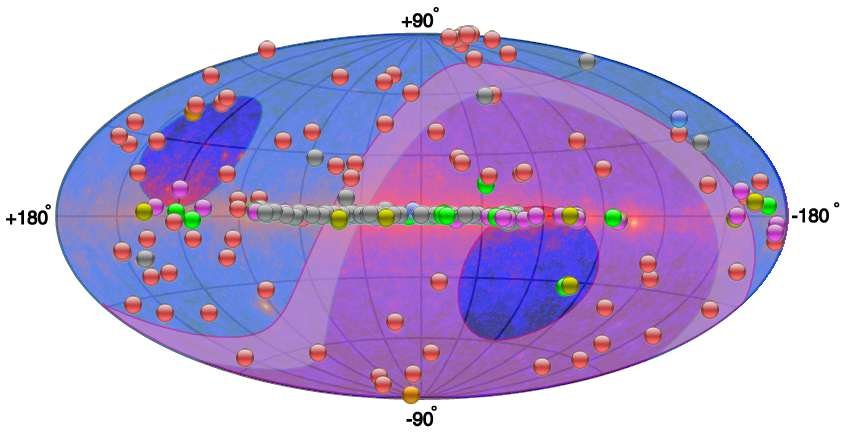
\includegraphics[width=\linewidth]{tevcat.pdf}
\endminipage\hfill
\minipage{0.15\textwidth}
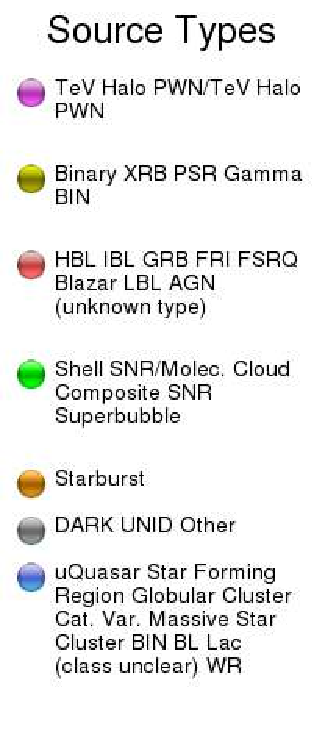
\includegraphics[width=\linewidth]{Pictures/legend_tevcat.pdf}
\endminipage\hfill
\caption{\label{fig:tevcat}Full skymap from TeVCat\cite{2008tevcat} catalog as of July 2019, with all the detected TeV sources. In the background, the \textit{Fermi}-LAT skymap is shown and the shadowed regions correspond to the \gls{magic} field of view (blue) and \gls{hess} (pink). }
\end{figure}

\subsection{Galactic sources}

As shown in figure \ref{fig:tevcat}, the richest region in $\gamma$-ray sources is the galactic plane, meaning that the majority of detected emitters belong to our galaxy. In this section, the different characteristics of these sources will be described. 

\subsubsection{Pulsars} \label{sec:pulsars}

Pulsars are the most common type of $\gamma$-ray emitters known. When a massive star ($< 8 M_{\odot}$) suffers gravitational core collapse at the end of its life, the resulting object is a compact neutron star sustained by degeneracy pressure, where neutronization (the combination of protons and electrons) has taken place due to the extremely high pressures which lead to high densities ($> 10^{9}g/cm^{3}$). The neutron star comprises 1 - 2 $M_{\odot}$ in a radius of 10 - 14 km and as the angular momentum of the parent rotating star is conserved, the much more compact neutron star will spin at extremely high velocities  with periods  that can go from milliseconds to a few seconds. This fast spin produces strong magnetic fields in their surroundings where electrons and positrons are accelerated by the electric field aligned with the magnetic field. When the magnetic fields are aligned with the line of sight from the Earth, we can detect a pulsed emission (mainly synchrotron and curvature radiation) with the period of the rotation of the neutron star, and the object is called a pulsar. Pulsed emission from this kind of object has been detected a broad band in the electromagnetic spectrum, from radio to $\gamma$-rays.\\ 
It is generally accepted that the origin of the $\gamma$-ray emission from pulsars is due to curvature radiation, produced when relativistic electrons accelerated in gaps of the electromagnetic fields powered by the pulsar rotation, are trapped and propagate along the lines of the magnetic field \cite{2008crabmagic}. However, the location of the gaps and the dominating acceleration mechanism are not well known and there are different models proposed (see figure \ref{fig:crabpulsar}).\\ 

\begin{figure}[!htb]
\minipage{0.4\textwidth}
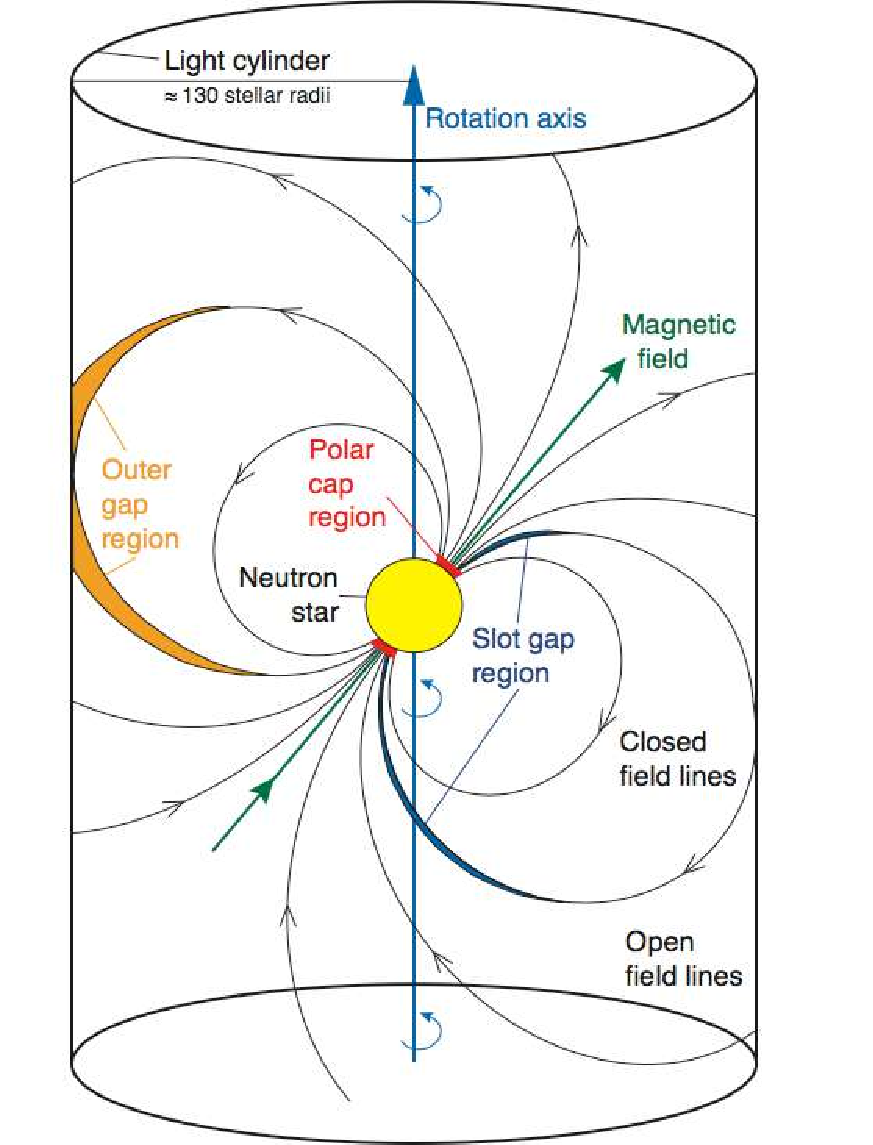
\includegraphics[width=\linewidth]{Pictures/pulsargaps.pdf}
\endminipage\hfill
\minipage{0.6\textwidth}
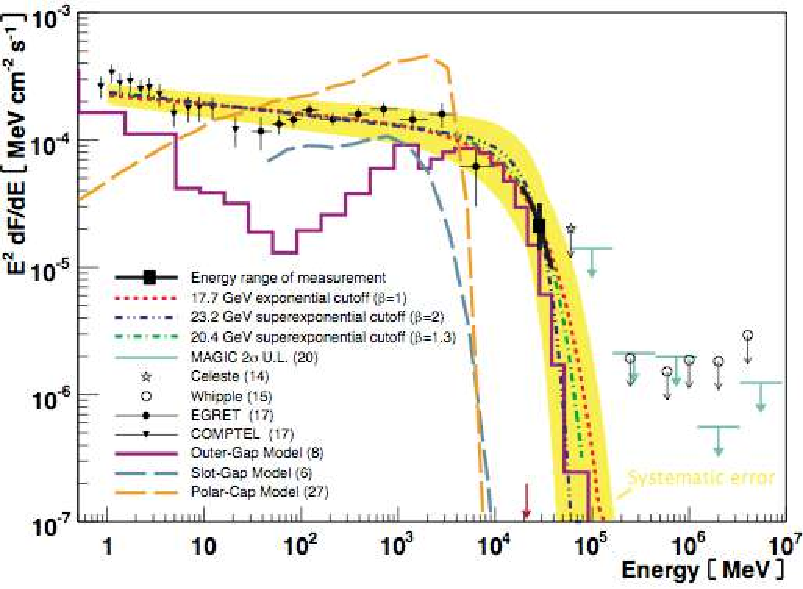
\includegraphics[width=\linewidth]{Pictures/crabcutoff.pdf}
\endminipage\hfill
\caption{\label{fig:crabpulsar} \textit{Left:} Crab pulsar's magnetosphere where the location of the three models (Polar-Cap in red, Slot-Gap in blue and Outer-Gap in yellow) is shown. \textit{Right}: Crab pulsar spectral cutoff. Figures from \cite{2008crabmagic}}
\end{figure}

Combined observations of the Crab pulsar from the \gls{comptel}, the \gls{egret} \cite{2001CrabCOMPTEL}, \gls{magic} \cite{2008crabmagic}, \gls{veritas} \cite{2013CrabPulsarVeritas} and \textit{Fermi}-LAT \cite{2010FermiCrabPulsar} have shown that their spectrum follows a power law with a cutoff at energies over a few GeV (see figure \ref{fig:crabpulsar}). The detection of the pulsar emission at energies over 25 GeV by \gls{magic} ruled out the possibility of acceleration happening too close to the pulsar (as the Polar-Cap model assets) because the magnetic pair-production attenuation would provide a super-exponential cutoff at much lower energies to those observed. Currently, the Outer-Gap model offers the best explanation of the observed Crab spectrum \cite{2008gapmodels}.\\
While pulsars are the most common $\gamma$-ray emitters, only two have been detected in the \gls{vhe} range, up to TeV energies: the Crab and Vela pulsars \cite{Gajdus2016The}. 

\subsubsection{Supernova Remnants}\label{sec:SNRs}

Supernovae are the result of the evolution of a star, which suddenly becomes much brighter while shells of gas are expelled off to the interstellar medium in an explosive event. They can be classified in different types by features in their spectrum which also implies a different origin of the explosion. Type II supernovae show hydrogen emission lines, meaning they come from very massive stars ($M > 8 M\odot$) with hydrogen in their outer layers. After burning lighter elements (H, He, etc.) into heavy nuclei, fusion reactions become inefficient and the imbalance between gravitational forces and pressure radiation lead to the collapse of the central core into a neutron star or a black hole in a violent reaction, expelling shells of material at high velocities. Type I supernovae do not present hydrogen lines, meaning they come from a hydrogen-poor star. They usually are produced by white dwarfs in binary systems which accrete material until reaching the Chandrasekhar limit \cite{1931Chandra} and suffer a thermonuclear explosion. Type I supernovae are classified in subtypes: Type Ia show Si lines in their spectra, whereas those without these lines are classified as Ib if they have He lines and Ic if not \cite{2006osterbrock}.\\
The structure of ejected material which is left in the surroundings of the parent star is the \gls{snr}. These structures can be classified in different types depending on their spectrum, but the most important feature to differentiate them is the presence (or not) of a shell. There are shell-type \gls{snr}, in which the material in the surroundings is heated by the power of the shockwave during the \gls{sn} explosion. The so called \textit{plerion} \gls{snr} or \gls{pwn} do not present a shell. The result of the \gls{sn} explosion is always a central pulsar and their emission is produced by the interaction between electrons ejected to the medium by the pulsar and its huge magnetic field. There is also a composite type of \gls{snr} where a plerion is surrounded by a shell and depending on the wavelength observed, they emit more like one type or the other \cite{1988SNR}.\\
Depending on the \gls{snr} type, the  particle acceleration and $\gamma$-ray emission would have a different origin and features.\\

\begin{itemize}
    \item \textbf{Shell-type remnants:} Shell-type remnants, the commonly referred simply as \glspl{snr}, are the most popular candidates for \gls{cr} acceleration. \glspl{cr} are deflected by magnetic fields in the \gls{ism} which makes it impossible to trace back the emission direction, but neutral particles, like neutrinos and $\gamma$-rays coming from \glspl{snr} can be used as tracers of \gls{cr} acceleration.
    We know \glspl{cr} can produce $\gamma$-rays via hadronic interactions with the gas and dust in the medium. For example, the production of pions and posterior pion decay would give rise to a spectrum with a characteristic peak at 67.5 MeV, if pions are at rest. \\
    A simple energetic argument is used to pose shell type remnants as the main source of galactic \glspl{cr}. As a rough estimation, if we assume that the typical total kinetic energy produced by a \gls{sn} explosion is around $E_{SN} \sim 10^{51}$ erg, with a \gls{sn} rate in the galaxy of about one in 50-100 years, and a constant fraction $\eta$ of the kinetic energy is transferred to hadrons, it can be shown that this fraction has to be of the order of the 10\% to retrieve the approximated \gls{cr} luminosity in the galaxy $L_{CR} \sim 2 \times 10^{41}$ erg/s.
    \begin{equation}
        L_{CR} = \eta \cdot E_{SN} \cdot SN_{rate} = 0.1 \cdot 10^{51} erg \cdot 50 yr^{-1} \propto 10^{41} erg/s
    \end{equation}
    
    A more detailed analysis using real data of galactic \gls{snr} was done by \cite{2016originCR} arriving at the conclusion that future $\gamma$-ray data can be used to constrain the amount of \gls{cr} energy coming from \gls{snr}. However, there are still problems on proving this hypothesis because many of the $\gamma$-ray signatures coming from \gls{snr} have a leptonic origin rather than hadronic. Also, for \gls{snr} to reproduce the full spectrum of \gls{cr}, \glspl{snr} should be pevatrons (meaning they can accelerate \gls{cr} to PeV energies) at some fraction of their lifetimes, to reach the region after the \textit{knee}. Still, no \gls{snr} pevatron has been observed yet but high hopes are deposited in the next generation of $\gamma$-ray experiments \cite{2018SNRPevatrons}.
    
    \item \textbf{Plerions or Pulsar Wind Nebulae}. As mentioned, \gls{pwn} are powered by a central rotating pulsar which dissipates kinetic energy over time in the form of \textit{spin down luminosity}. This energy is injected steadily into the surrounding nebula of ejected material that was formed during stellar evolution. To understand the features of the emission of \gls{pwne}, it is important to follow their evolution with time and how the period, spin down luminosity and magnetic field changes \cite{2006PWNe}. A pulsar is formed in a \gls{sn} explosion and the final state of the pulsar and its \gls{pwn} will depend on how it interacts with the \gls{snr}. If the \gls{snr} expands outward freely, the pulsar will remain in the center, but if a reverse shock happens, reverberations between the \gls{pwn} and the shock can produce instabilities which in the end will displace the pulsar from its original position, even being able to cross away the \gls{snr} shell.\\
    Strong magnetic fields in pulsars create currents of particles of the surrounding nebula, producing pulsar winds. Electrons accelerated this way produce synchrotron radiation from radio to X-ray wavelengths. The wind starts decelerating when reaching the nebula radius, due to the more slowly expanding material and thus a wind termination shock is formed. The TeV $\gamma$-ray emission from \gls{pwne} is explained as \gls{ic} emission produced by the relativistic particles in the shocked wind interacting with the synchrotron photons.
    The Crab \gls{pwne} was the first source detected of this type, associated with a \gls{sn} explosion observed in 1054CE, and has become a sort of standard candle for $\gamma$-ray astrophysics.\\
    
    \item \textbf{Composite remnants}. A rare type of \gls{snr} is a combination of the previous two, where a \gls{pwn} is surrounded by a shell-type \gls{snr}. Usually, \gls{pwn} are considered young \glspl{snr} while shell-types are older systems. Composite \glspl{snr} could be an intermediate phase of evolution where the shell and the \gls{pwn} evolve and interact together \cite{2014compositeSNRhess}. In these systems, the \gls{pwn} formed in the interior of the \gls{snr} expands outwards and it can encounter the inward reverse shock of the \gls{snr} \cite{2015SNRingammarays}. Some examples of this kind are \glspl{snr} W28, W44 and SNR G21.5-0.9, which is shown in figure \ref{fig:compositesnr}. \\
\end{itemize} 

\begin{figure}
\centering
 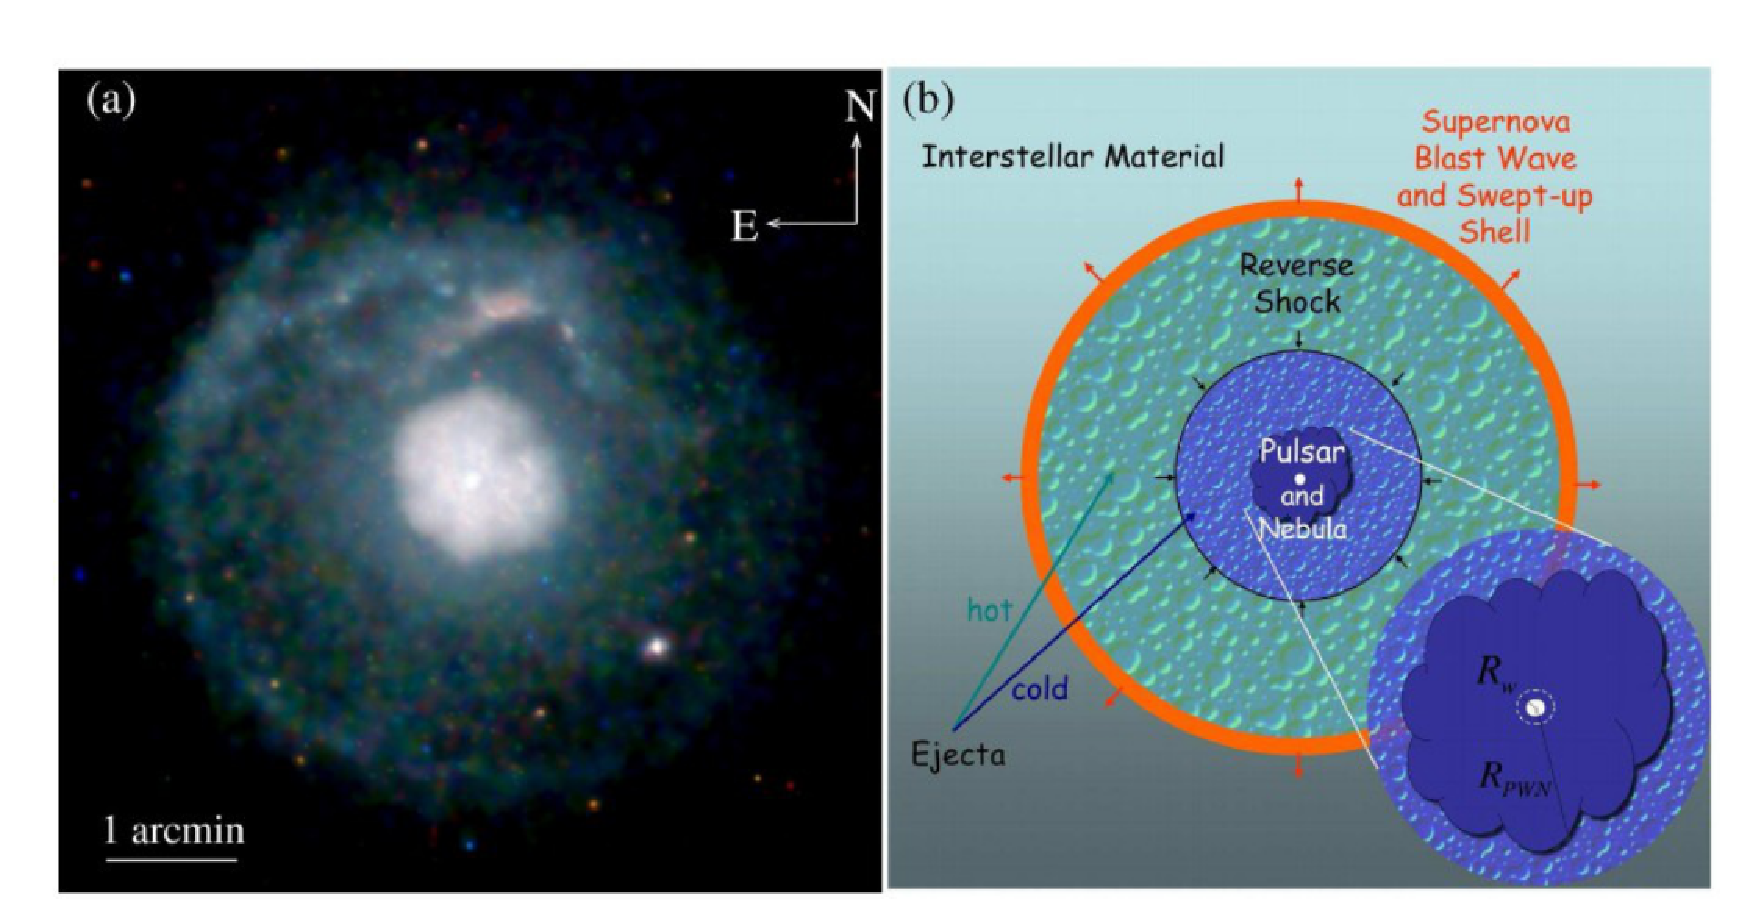
\includegraphics[width=0.77\textwidth]{Pictures/compositesnr.pdf}
  \caption{a): Chandra X-ray image of the composite \gls{snr} G21.5-0.9. b): Diagram of a \gls{pwn} inside a \gls{snr}. Pictures from \cite{2015SNRingammarays}.}
    \label{fig:compositesnr}
\end{figure}


\subsubsection{$\gamma$-ray binaries}

$\gamma$-ray binaries are systems composed by two objects orbiting each other: One is a compact object, such as a pulsar and the other can be an ordinary massive star big enough to reach the Roche lobe of the pulsar and so stellar winds connect the two objects. Just a few objects ($< 10$) of this kind have been detected in \gls{he} and \gls{vhe} $\gamma$-rays very recently \cite{2017gammarybinariespop}, and yet the exact mechanisms of the origin of their emission are unknown.
There are two main explanations to the \gls{he} and \gls{vhe} emission in $\gamma$-ray binaries. It can be produced by accretion energy released in the form of relativistic jets, or on the other hand, by the energy emitted by the pulsar in the form of pulsar winds in a similar way as in \gls{pwne}. The first case is denominated the \textit{microquasar} scenario due to its similarities with \gls{agn} (also known as quasars) but emitting jets in a smaller scale. However, a variety of indirect evidences seem to favour the pulsar wind interpretation mainly based in the spectral similarities of the known binaries with the power of a pulsar spindown. Also the presence of strong magnetic fields and morphological characteristics of radio emission are similar features to those found in \gls{pwne} \cite{2013binaries}. 

\subsubsection{Novae}

Binary star systems are rather common objects in the universe. One of the stars can be more massive than the other, evolving faster and becoming a white dwarf while the second star can still be in its main sequence phase. If this happens, the white dwarf can start to accrete material from the companion, building an accretion disk. The hydrogen rich gas in the surface of the white dwarf starts heating the bottom layers which becomes electron-degenerate, leading to a chain of thermonuclear explosions \cite{bode_evans_2008}. This event is known as "classical nova".
When the companion star is a red giant, which has highly increased its volume, the system is called a \textit{symbiotic binary system}. In this case, the interaction between the stellar wind of the red giant and the white dwarf surface expansion give place to a favorable scenario for particle acceleration.
 Both classical novae and symbiotic systems have been detected in \gls{he} $\gamma$-rays by \textit{Fermi}-LAT \cite{2010symbioticfermi}, \cite{2014fermiclassicNovae} although these results do not allow to differentiate between the different emission scenarios.\\
 
 \begin{figure}[!htb]
\minipage{0.45\textwidth}
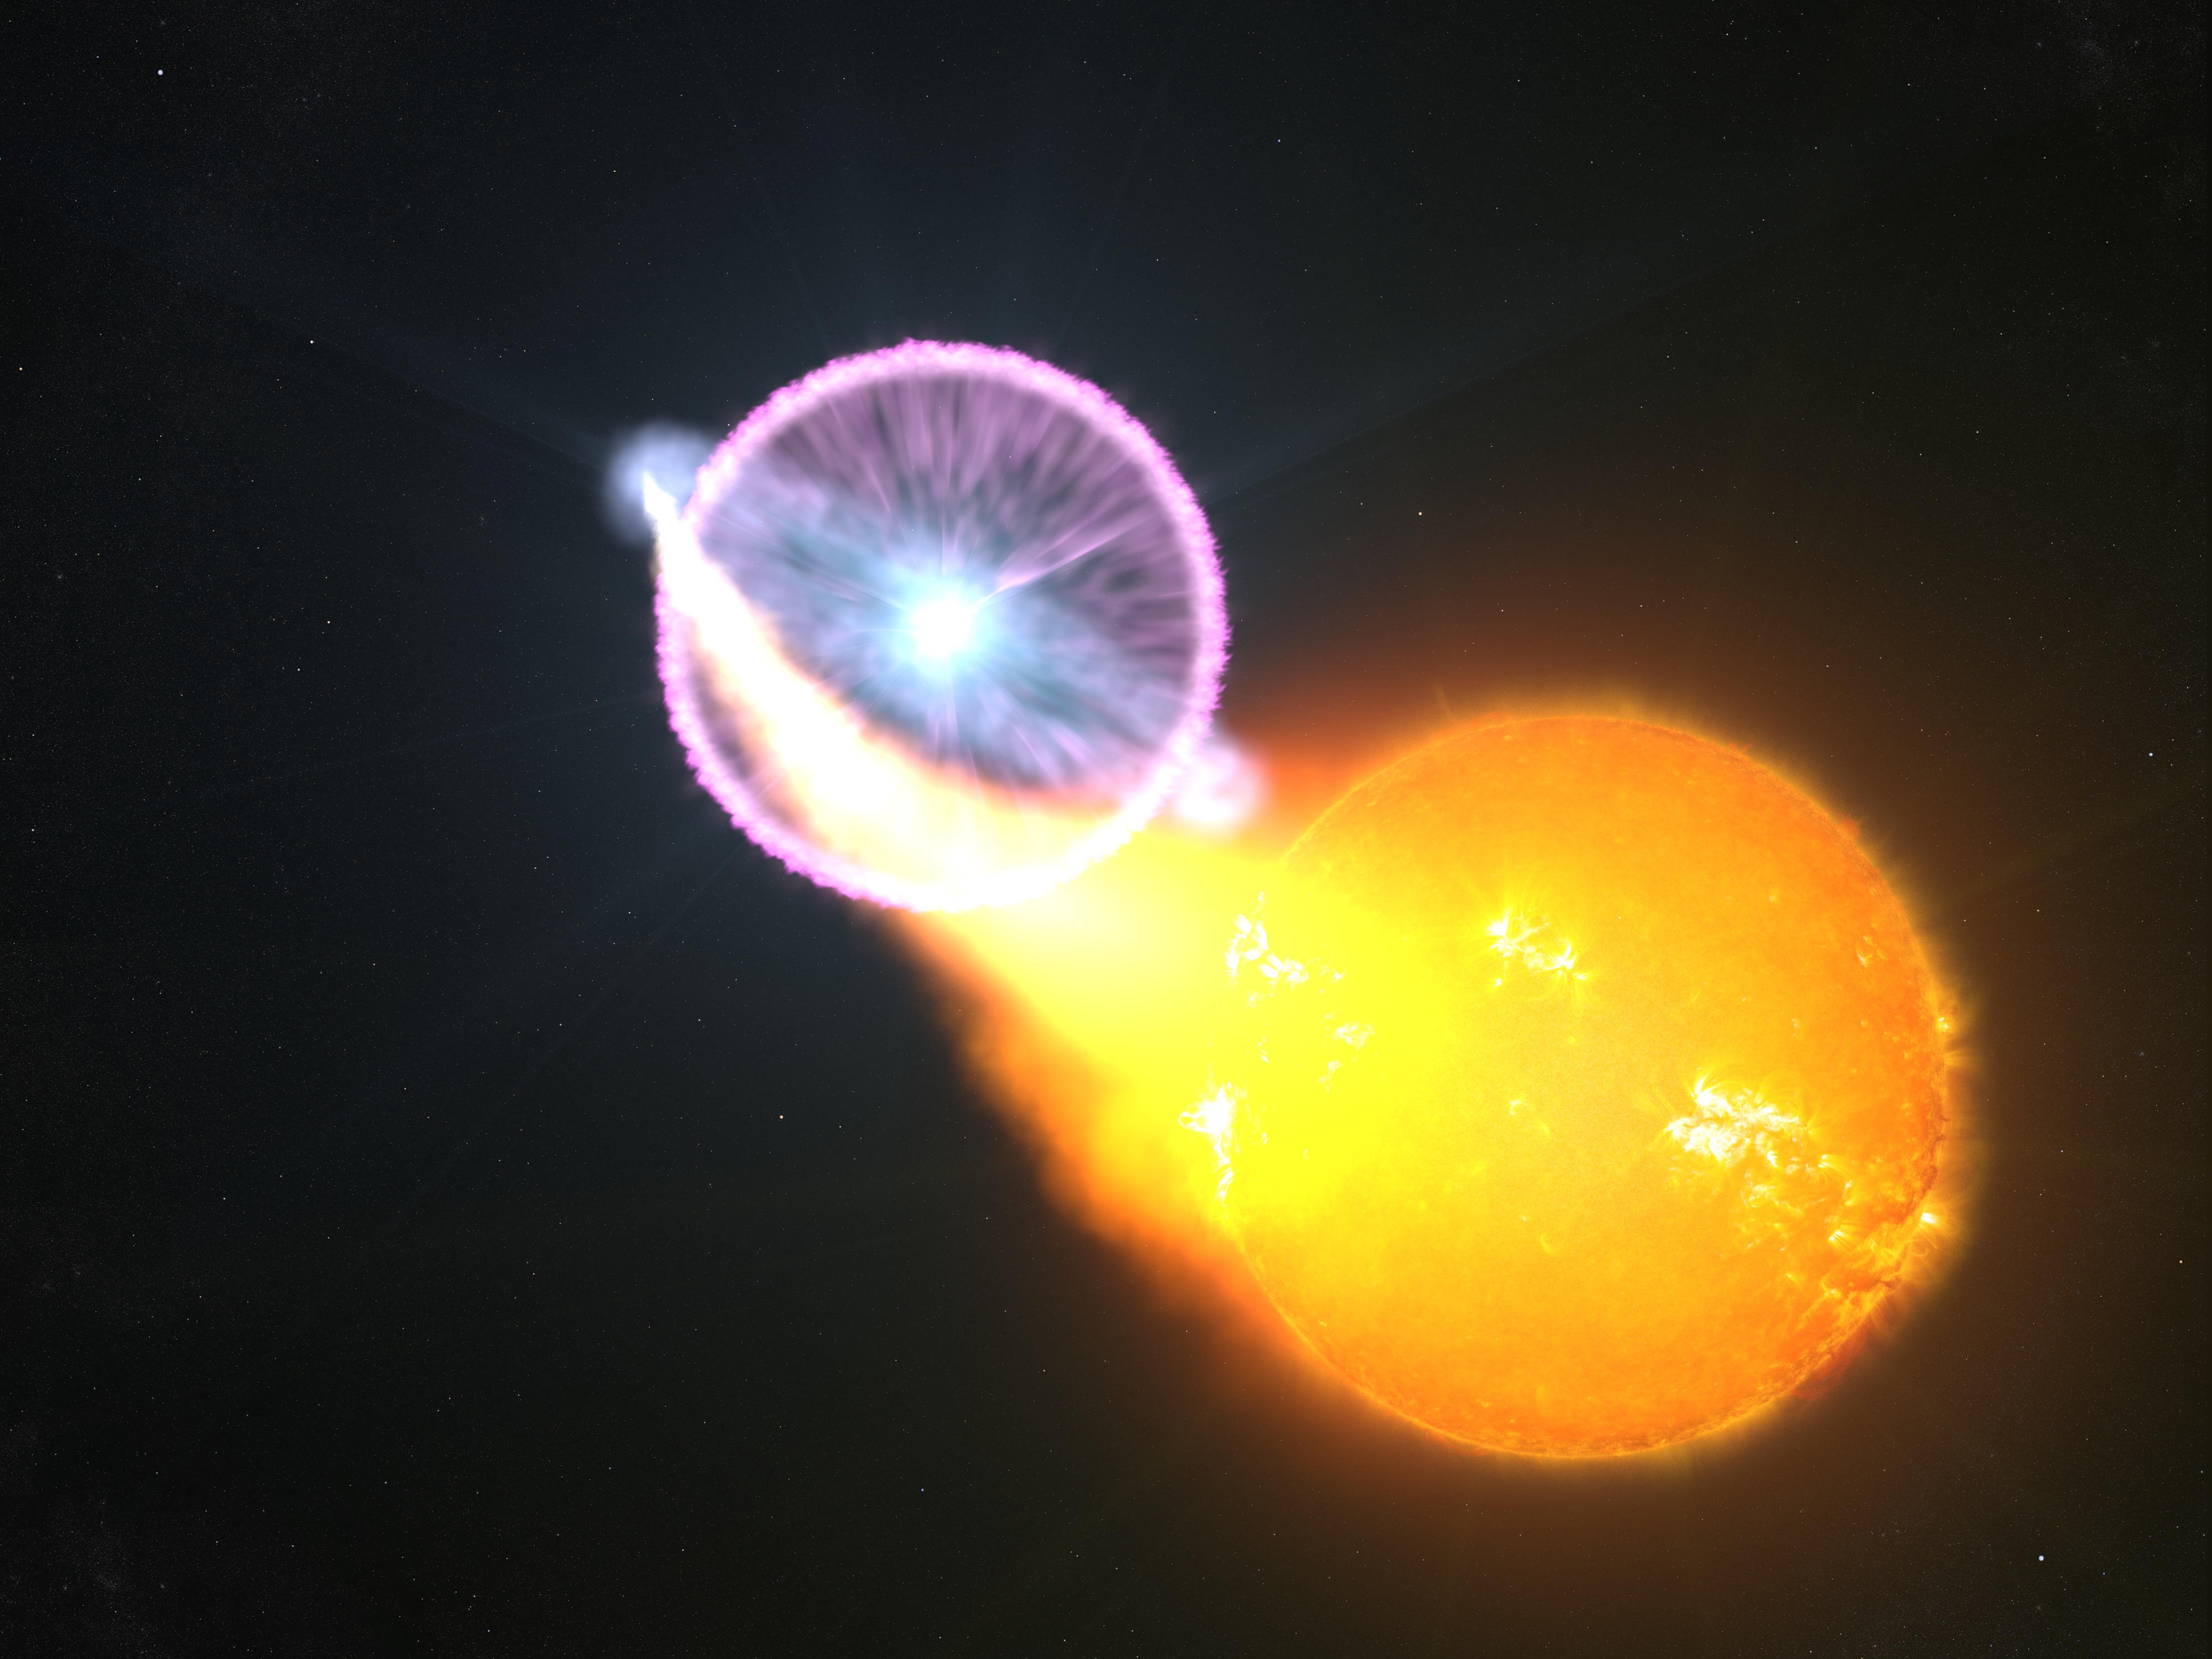
\includegraphics[width=\linewidth]{classical_nova_final_0.jpg}
\endminipage\hfill
\minipage{0.45\textwidth}
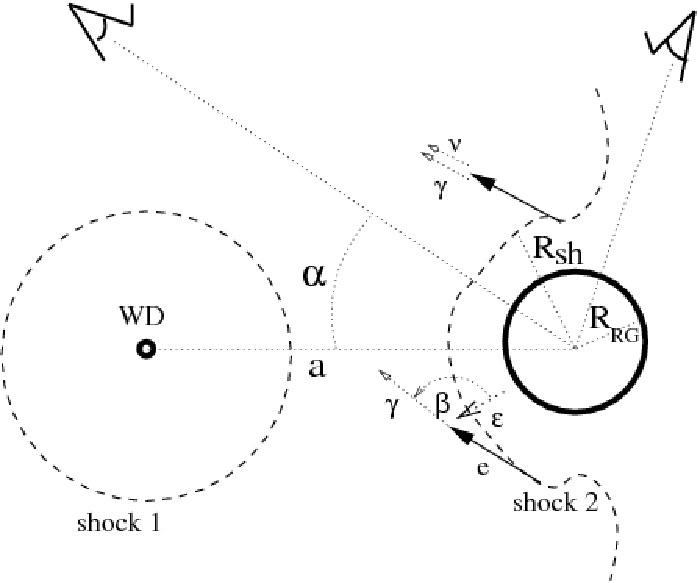
\includegraphics[width=\linewidth]{novadiagram.pdf}
\endminipage\hfill
\caption{\label{fig:novae} \textit{Left:} Artist concept of a classical nova. Credits: NASA's Goddard Space Flight Center/S. Wiessinger. \textit{Right:} Diagram of the geometry of the symbiotic binary system V407 Cyg from \cite{2012novagammaneutrinos}. The expanding shock (1) from the white dwarf partially overtakes the Red Giant (shock 2), producing particle acceleration through \gls{ic} (leptonic scenario, with angle of interaction $\beta$) and proton collisions with the red giant wind (hadronic scenario).}
\end{figure}

\subsubsection{The Galactic Center and the Fermi Bubbles} \label{sec:GCFermiBubbles}

The center of the Milky Way, known as the \gls{gc}, is a region of the sky situated at 4º longitude, 2º latitude, with a size of 600 x 300 pc and at a distance of about 8 kpc. It is obscured by dust in the optical and ultraviolet range, but emission in infrared, radio, X-rays and $\gamma$-rays reveals a prolific region full of energetic sources. Among many \glspl{snr}, \gls{pwne} and stellar clusters in HII regions, there is also a \gls{smbh}, Sagitarius A*, whose detection has been one of the major motivations for \gls{gc} surveys. Many $\gamma$-ray experiments have surveyed the \gls{gc} region (\textit{Fermi}-LAT , \gls{magic} \cite{2006GCMAGIC}, \gls{hess} \cite{2018GPHESS}, \gls{veritas} \cite{2016GCveritas}) and emission from HE to VHE bands has been detected. The main problem with this highly populated region is the difficulty of tell apart individual sources, making it a big challenge to identify the actual emission from  Sgr A* \cite{2011GC}. The high energy emission from Sgr A* has its origin in the strong winds produced by the presence of an accretion disk surrounding the black hole, where material is accelerated at very high energies \cite{2007GC}.\\

Closely related to Sgr A* might be the \textit{Fermi bubbles}, two large $\gamma$-ray lobes that appear to be ejected from the center of the galaxy. They were discovered while searching for a $\gamma$-ray counterpart to the \gls{wmap} haze \cite{2010Afbubblesdiscovery}, which is a residual microwave emission that arises after subtracting all the other known emission components. They extend to 55º up and above the \gls{gc} and are not symmetric, with an enhanced emission towards the south-east side of the bubbles. With well defined edges, an uniform power-law spectrum of index $\sim 2$ and a cocoon-like shape, they resemble jet-like structure \cite{2014Fbubbles}. Their origin is still under debate: They could be jets, outflows or the result of accretion events from the black hole, winds from \gls{sn} explosions or the remanent of \gls{agn} activity in the Milky Way in the past. \\

\begin{figure}[!htb]
\minipage{0.45\textwidth}
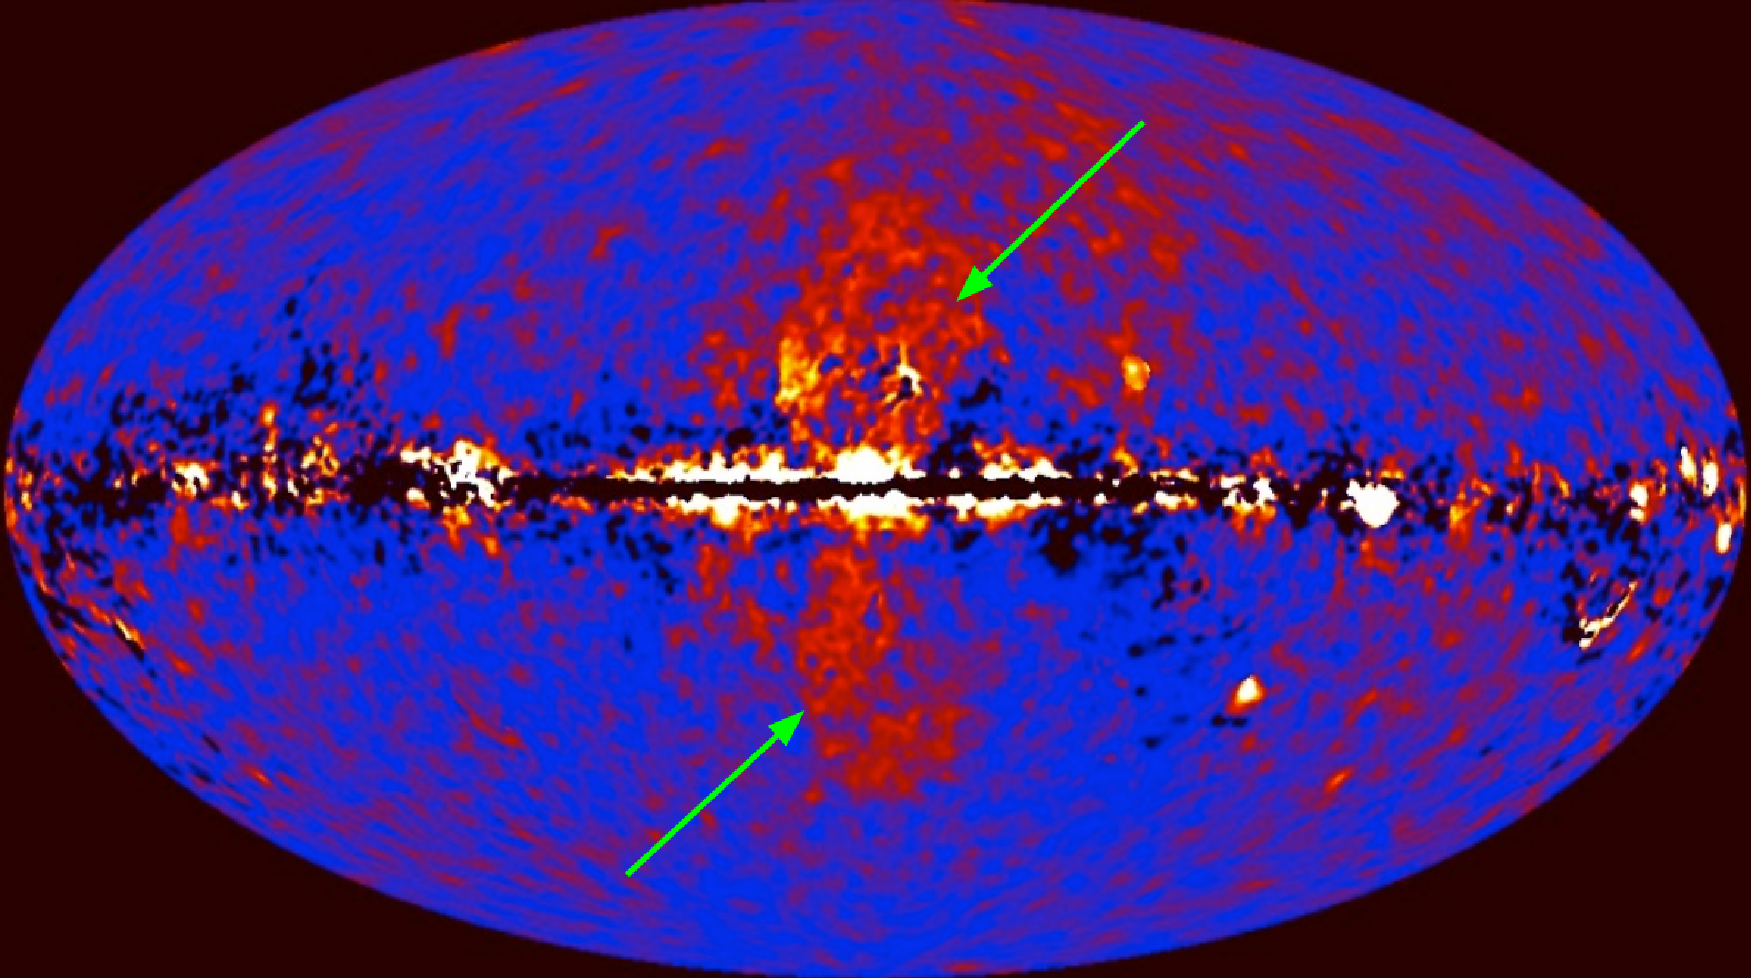
\includegraphics[width=\linewidth]{Pictures/fermi_bubb_arrows.pdf}
\endminipage\hfill
\minipage{0.45\textwidth}
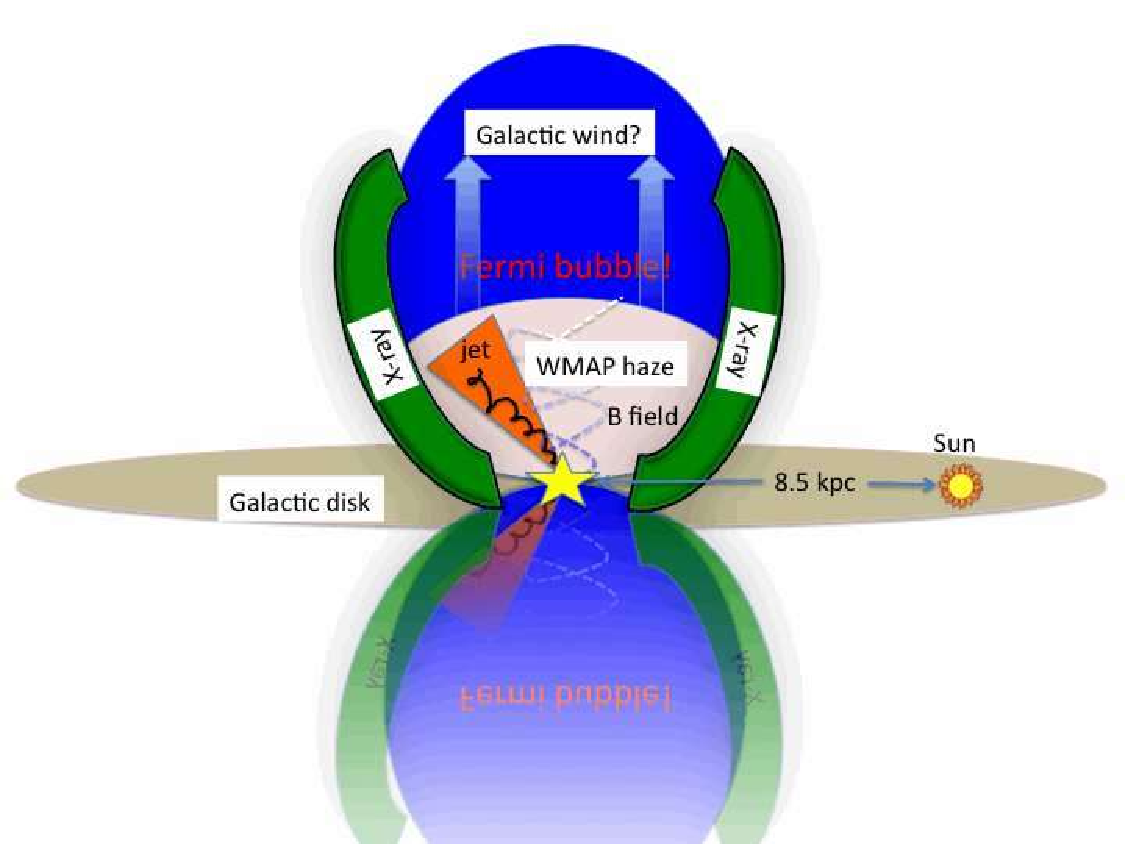
\includegraphics[width=\linewidth]{Pictures/diagramfbubbles.pdf}
\endminipage\hfill
\caption{\label{fig:fbubbles} \textit{Left:} The Fermi Bubbles as seen by \textit{Fermi}-LAT after subtracting all the other known $\gamma$-ray components. Credits: NASA/DOE/Fermi LAR/D. Finkbeiner et al. Right: Schematic picture of Fermi Bubbles structure from \cite{2010Afbubblesdiscovery}.}
\end{figure}

\subsubsection{Globular Clusters}

Globular clusters are compact gravitationally bounded stellar associations with spherical geometry which are distributed outside the galactic plane, conforming a spherical halo around the galaxy. They are old highly evolved systems with many compact objects like neutron stars, white dwarfs and pulsars even forming binary systems. Furthermore, the majority  ($\sim 80\%$) of \glspl{msp} (pulsars with a period of the order of milliseconds) detected up to date have been found in globular clusters.\\
Since all the mentioned objects are well known $\gamma$-ray emitters, globular clusters have been observed and  detected in $gamma$-rays by \textit{Fermi}-LAT \cite{2010globularclusterspopulationfermi} and \gls{hess}  \cite{2013globularclustersHESS}. Even pulsed $\gamma$-ray emission have been observed from individual \glspl{msp} \cite{2011detectionpulsationglobularcluster}, \cite{2013PulsedemissionfromGlobularM28}. 
Two types of models of $\gamma$-ray emission have been discussed to happen in globular clusters, both related to \glspl{msp}. One takes place in \glspl{msp} magnetospheres, where $\gamma$-ray emission would be produced by curvature radiation. The second type of models involve \gls{ic} scattering of electrons accelerated close to the \gls{msp} with optical, infrared or CMB photons \cite{2016GlobularClustersFermi}.  
\subsection{Extragalactic sources}

While most of the $\gamma$-ray emission detected on Earth comes from the galactic plane, there is a big amount of individual sources outside our galaxy which produce \gls{he} radiation and allow the study of a new range of extragalactic phenomena. A big caveat for extragalactic sources is that the \gls{vhe} range is suppressed by the \gls{ebl} absorption, as described in section \ref{sec:absorption}.

\subsubsection{Active Galactic Nuclei}

\gls{agn} are the brightest steady sources of $\gamma$-ray in the universe and the most luminous known electromagnetic emitters. Known as \textit{black-hole galaxies}, their strong emission is powered by infalling gas into a massive \gls{bh} located in the center. The \gls{bh} attracts gas and material from the galaxy forming an accretion disk, where matter loses angular momentum through viscous and turbulent processes, and emits a huge amount of energy from ultraviolet to soft X-ray bands \cite{1995AGN}. \gls{agn} can be classified in two broad types, according to their radio emission: \textit{Radio-quiet} and \textit{radio-loud}. Further observational classification depends strongly on the orientation angle, which can make \glspl{agn} appear as spectroscopically completely different sources, depending on the region of the object that is showing. All \gls{agn} have a dusty tori, broad-line regions, narrow-line regions and strong blue/UV bump emissions from the accretion disk \cite{2016AGNsingammarays}. Depending on the angle, one or several of these regions will be observable and will show their particular features in the spectrum. Figure \ref{fig:schemeAGN} show a scheme of AGNs taxonomy.\\
Radio-loud \gls{agn}, also known as \textit{blazars}, are about three orders of magnitude brighter in radio band than their quiet counterparts. This radio emission is directly related with the presence of relativistic jets of plasma which carries a big part of the energy released during accretion and that afterwards is emitted as radiation from radio to $\gamma$-rays \cite{2016AGNgammarayobss}. They are associated with elliptical galxies that have undergone recent mergers.
On the contrary, radio-quiet galaxies doesn't show jets and so do not account for high energy non-thermal emission. Also, they are typically spiral galaxies in lower density regions \cite{1995AGNradioloudradioquiet}.
Blazars are rare among \gls{agn}, accounting only for 10\% of the total, but a large number of them has been detected in $\gamma$-rays, with more than 1500 sources detected at GeV energies, and more than 60 at TeV energies \cite{2016AGNsingammarays}.

\begin{figure}
  \centering
  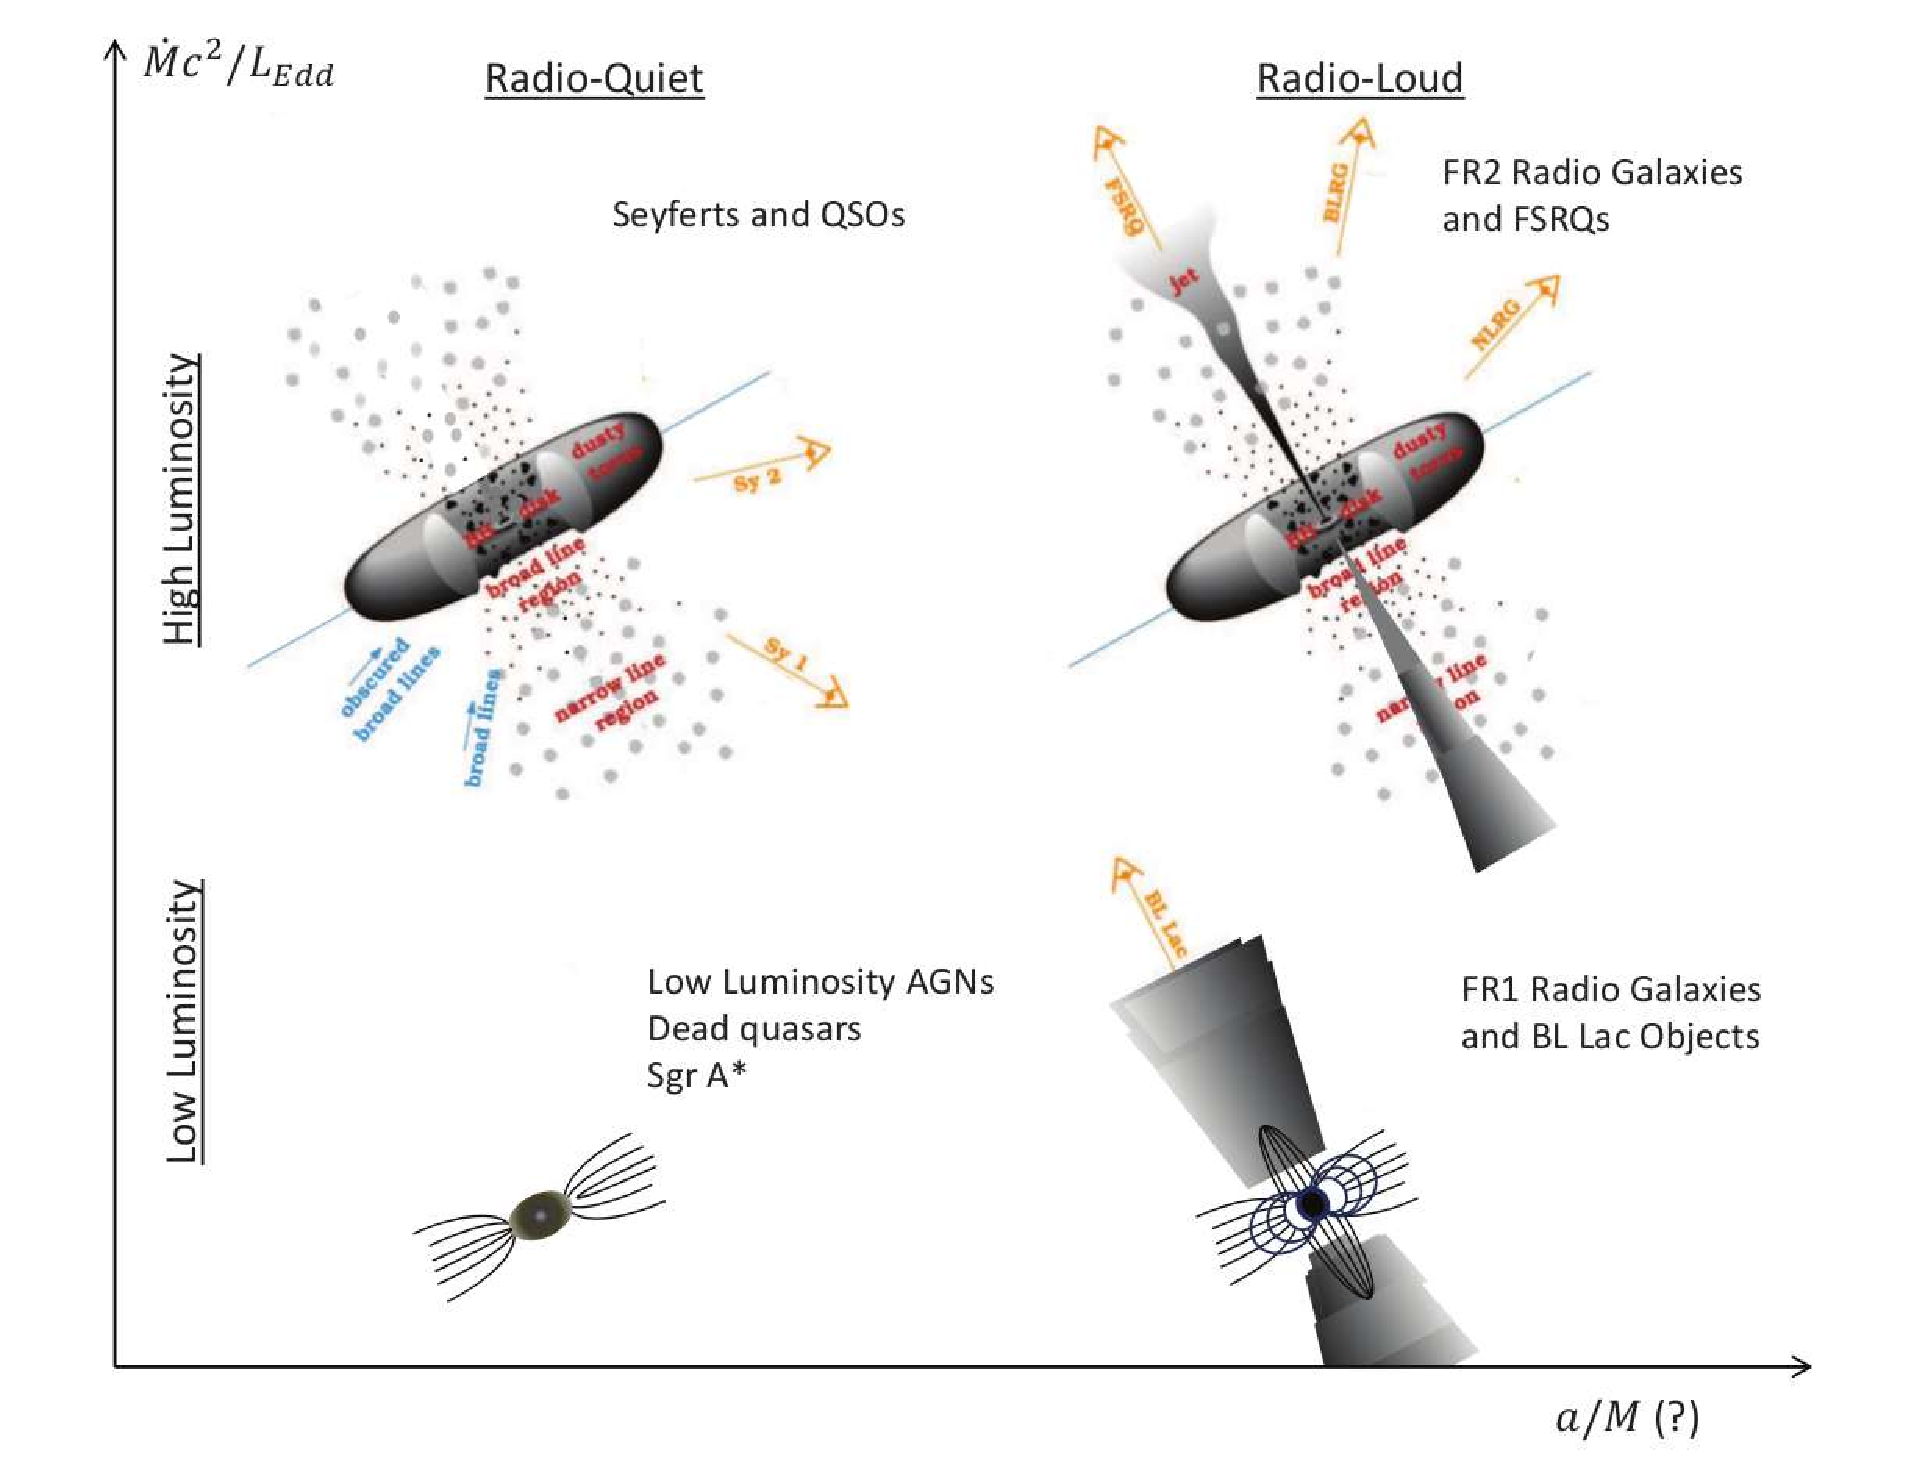
\includegraphics[width=\textwidth]{Pictures/schemeAGN.pdf}
  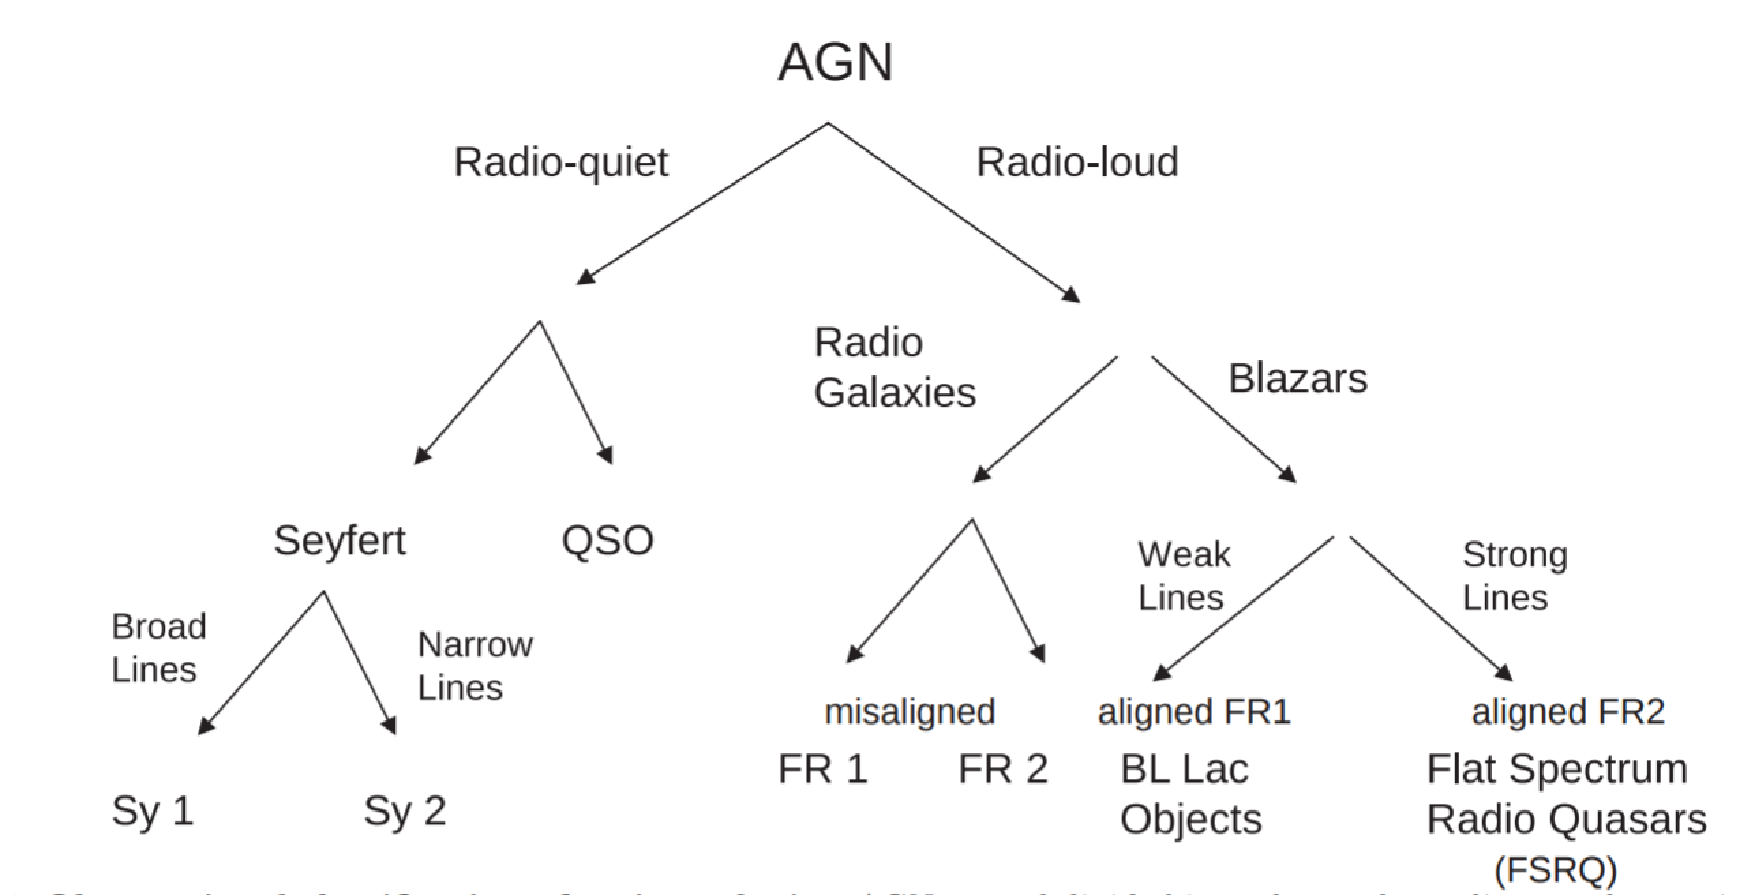
\includegraphics[width=\textwidth]{Pictures/AGNclassification.pdf}
  \caption{Left: AGN taxonomy as from \cite{2016AGNsingammarays}. In this scheme, the vertical axis represents the luminosity power in terms of the mass-acretion rate and horizontal axis represents the \gls{bh} rotation. Right: Observational calssificartion of active galaxies. QSO= quasi-stellar objects; Sy1(Sy2) = Seyfert 1(2); FR1(FR2)=Fanaroff-Riley 1(2). Pictures based on \cite{1995AGNunifiedschemes} from \cite{2016AGNsingammarays}.} 
  \label{fig:schemeAGN}
\end{figure}

\subsubsection{Gamma Ray Bursts}

\glspl{grb} are short and intense flashes of $\gamma$-ray emission coming isotropically from random directions in the sky. With a range of luminosities from $10^{51} ergs/cm^2$ to $10^{52} ergs/cm^2$ they are the brightest transient objects in the sky \cite{2004GRB}. They can be classified by their duration, havign two distinct populations: short \glspl{grb}, which last just a few seconds; and long \glspl{grb} which can last for few minutes \cite{1993GRB2pop}. Long bursts are usually followed by afterglows in X-rays, optical and radio which can last for several years after the event.
The so called \textit{fireball} model is the generally accepted mechanism which drives \gls{grb} \cite{1999GRBfireball}. Since the observed emission of the bursts is not thermal, its origin must be the result of the conversion of an ultra-relativistic  energy flow into radiation in an optically thin region. The energy flow could come from the kinetic energy of accelerated particles or electromagnetic Poynting flux. In this model, the process is ignited by an "inner engine" which is not possible to observe directly, but which activity can be characterized by the observed temporal structure of the bursts. The engine produces an explosive fireball of the size of the engine itself. There is an alternative model based in internal shocks, where the engine would produce a wind and a long energy flow. About the nature of the phenomena producing \glspl{grb}, there exist an apparent difference between the origin of short \gls{grb} and long \gls{grb} according on their hardness ratio (defined as the ratio of the flux in two separated bands) versus duration plot (see figure \ref{fig:GRB2classes}) \cite{1993GRB2pop}.\\

\begin{figure}
\centering
 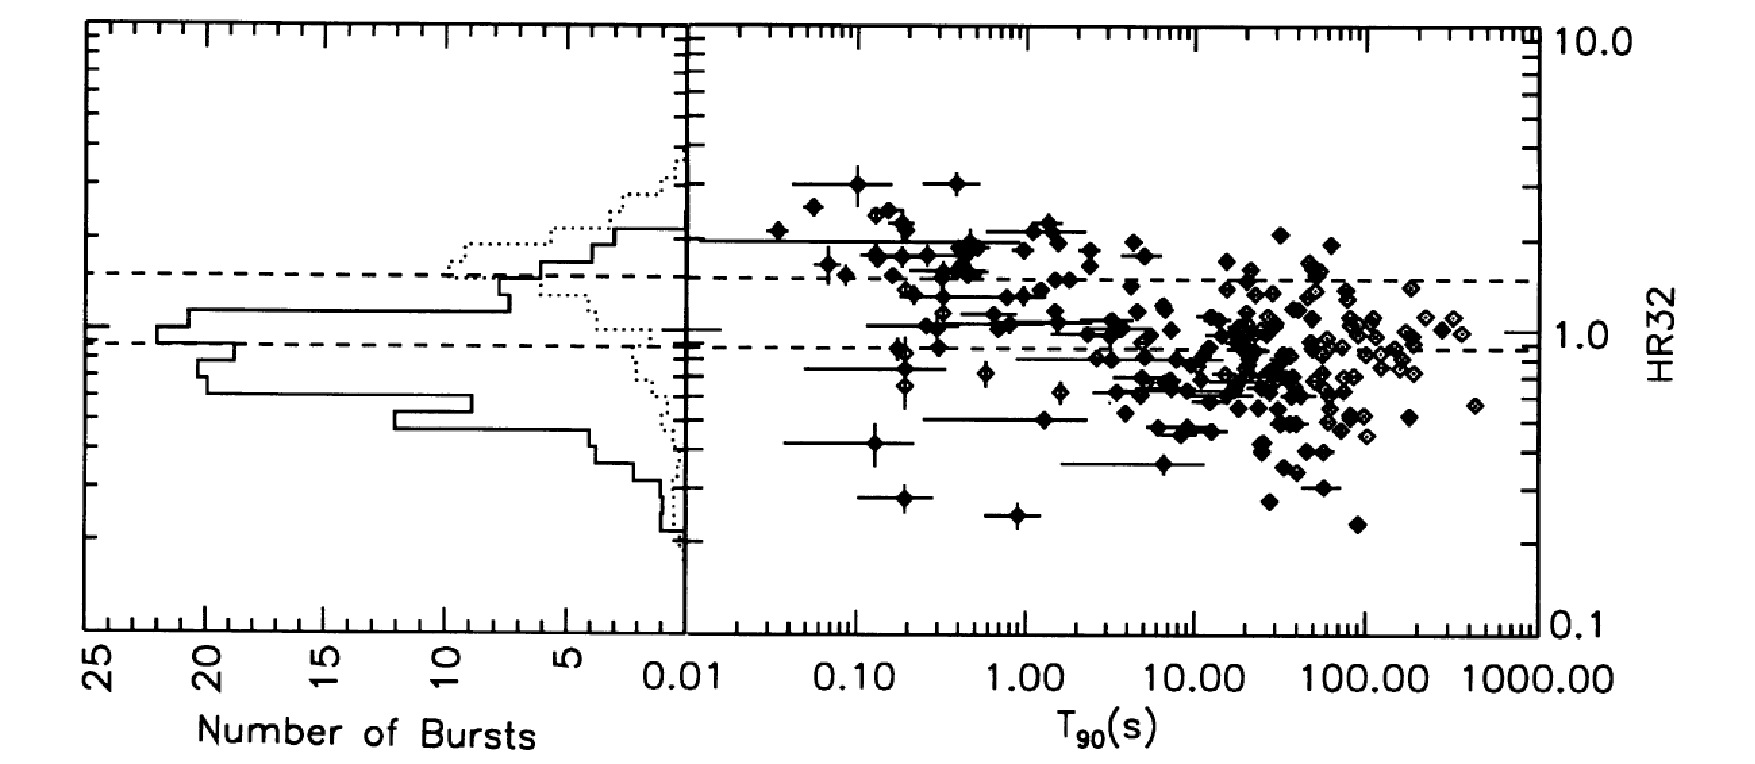
\includegraphics[width=0.77\textwidth]{Pictures/GRBhardnessdurationplot.pdf}
  \caption{\textit{Left:} Hardness ratios for the two duration classes of \gls{grb}. Solid lines corresponds to short \glspl{grb}, dashed line to long \glspl{grb}. \textit{Right:} Hardness vs. duration plot, where duration $T_{90}$ is defined as the time during which the cumulative counts > 25 keV increase from 5\% to 95\% above background. Dashed lines correspond to the mean hardness ratio of the two classes. Figure from \cite{1993GRB2pop}.}
    \label{fig:GRB2classes}
\end{figure}

These two populations in the hardness ratio vs. duration plot, together with rather significant spectral differences \cite{2015GRBorigin} and afterglow observations, suggest that long \glspl{grb} are closely related to star forming regions, compatible with \gls{sn} explosions of massive stars. Short \glspl{grb} on the other hand, could be related to more evolved regions and be the result of neutron star mergers, such as the recently detected gravitational wave event GW170817 by LIGO/VIRGO \cite{2017GW170817} which was also detected as a \gls{grb} by the Fermi Gamma-Ray Burst Monitor and later observed by \textit{Fermi}-LAT \cite{2018FermiGW170817}. Also recently \gls{magic}, which were specifically designed to observe such objects, detected the first event in the \gls{vhe} range \cite{2019MAGICGRB}.

\subsubsection{Starburst galaxies}

Starburst galaxies are those with a greatly enhanced star formation, whose \gls{sfr} is considered to be out of equilibrium, consuming gas for star formation at very short timescales (< 1 Gyr). Since the \gls{sfr} is highly correlated with the \gls{sn} explosion rate, it is expected that $\gamma$-ray emission detected from starburst galaxies has its origin in \glspl{snr}.\\
The production and transport of \glspl{cr} in the \gls{ism} significantly affects the star formation, because \glspl{cr} penetrate deep into molecular cloud cores (molecular clouds are dense gas regions where star formation takes place) catalyzing complex chemical reactions which can affect the initial conditions of star formation and evolution \cite{2016starburst}. The conditions of the \gls{ism} in starburst galaxies are very different from Milky Way \cite{2009starbursthess}. The gas density is much higher and the high population of massive stars produce a huge amount of radiation, which is absorbed by dust an re-emited in infrared. Magnetic fields are also affected by the presence of such population. Thereby particles accelerated in the region will suffer strong losses of energy and faster cooling. Detection of $\gamma$-rays from starburst galaxies is a key probe to understand the efficiency of \gls{cr} acceleration in \glspl{snr} and \gls{cr} transport in different \glspl{ism}.  \\
The current generation of $\gamma$-ray telescopes have detected NGC253 and M82 starburst galaxies (\cite{2009starbursthess}, \cite{2009starburstveritas}, \cite{2010starburstFermi}), which has been long predicted to emit $\gamma$-rays up to \gls{vhe} range.\\

\subsubsection{Galaxy clusters} \label{sec:clusters}

Galaxy clusters are the largest gravitationally bounded structures in the universe. They are mainly composed of \gls{dm} (70-80\% of the total mass) and their ordinary matter is composed by the galaxies and the filaments connecting them, plus a big amount of hot gas in the surroundings called the \gls{icm}\cite{2017galaxyclusters}. In the standard paradigm of structure formation, clusters are formed by hierarchical mergers and accretion of smaller structures. Mergers are the most energetic phenomena to occur in the universe (they release $10^{63}$-$10^{64}$ ergs/Gyr) and they dissipate energy in the form of shocks which heat the gas, or through large-scale \gls{icm} motions \cite{2014CRinClusters}. Part of the energy dissipated during this process is fused into particle acceleration to ultra-relativistic energies, thus they are a source of \gls{cr} production. Radio observations of galaxy clusters proves the existence of non thermal emission from synchrotron radiation processes in the \gls{icm}. Galaxy clusters can therefore be a source of \gls{he} photons which can be produced via leptonic scenario through \gls{ic} scattering of \gls{cmb} photons with ultra-relativistic electrons, or hadronic scenario by neutral pion decay.\\

Until recently, $\gamma$-ray experiments that tried to detect $\gamma$-ray signal from the closest galaxy clusters were only able to set upper limits \cite{2010LimitsClustersFermi}, \cite{2012LimitsClustersMagic}. \textit{Fermi}-LAT was able to report a detection of an extended $\gamma$-ray signal from the Coma cluster roughly correlated with the radio halo \cite{2018ComaCluster}.\\

\subsubsection{Neighbour galaxies}

The Local Group is the cluster of galaxies gravitationally bounded to the Milky Way. They are the closest galaxies to be observed and their characteristics are expected to be similar to those of our own galaxy. The second and third closest and spatially resolved galaxies (the first being the Canis Major dwarf galaxy) are the \gls{lmc} and the \gls{smc}. They are two irregular dwarf galaxies seen in the southern hemisphere, at a distance of 50 kpc \cite{2018LMCdistance}. They present a remarkable high star formation rate ($\sim 0.2$yr$^{-1}$ for the LMC, $0.3$yr$^{-1}$ for the SMC \cite{2014LMCSFR}, compared to the 0.68yr$^{-1}$ to 1.45yr$^{-1}$ of the Milky Way \cite{2010MilkyWaySFR} in a much smaller volume.). They can produce $\gamma$-ray emission due to the interaction of \gls{cr} with \gls{ism}.\\
The first detection of a $\gamma$-ray diffuse signal from the \gls{lmc} was made by \gls{egret} \cite{1992LMCEgret}, being the first normal galaxy outside the Milky Way detected in $\gamma$-rays. The \gls{smc} was first detected in $\gamma$-rays by \textit{Fermi}-LAT \cite{2010SMCFermi}. Further observations of the \gls{lmc} from \textit{Fermi}-LAT at \gls{he} \cite{2010LMCFermifirst}, \cite{2016LMCFermi6years}, \cite{2016LMCFermiBinary} and \gls{hess} \cite{2015LMCHess}, \cite{2012LMCHessfirst} at \gls{vhe} revealed a complex structure of the diffuse emission and a population of very interesting individual sources comprising pulsars, \glspl{snr}, \gls{pwne} and $\gamma$-ray binaries. Since the \gls{lmc} emission in $\gamma$-rays is one of the main topics of this thesis, it will be extensively treated in chapter ??.\\
Apart from the before mentioned starburst galaxies M82 and NGC253, other close galaxies such as M31 and M33 have also been observed and detected in \gls{he} $\gamma$-rays by \textit{Fermi}-LAT \cite{2017M31M33Fermi}. 

\subsection{Potential Dark Matter annihilation emission sources}

In section \ref{sec:DM} the production of $\gamma$-rays through \gls{wimp} annihilation or decay was described. In the search for this kind of signal, one can analyze which would be the best sources in the universe for an indirect search of \gls{dm}. First of all, they must have a high amount of \gls{dm}, given by the astrophysical parameter J-factor (integral term in eq. \ref{eq:flux}). Also, a low background of other $\gamma$-ray sources would allow to unequivocally identify the \gls{dm} signal. Following these premises, indirect \gls{dm} searches have been performed by $\gamma$-ray experiments in the most promising sources:\\

\subsubsection{Milky Way Galactic Center}

In the present evolutionary stage of the universe, galaxies are believed to be embedded in \gls{dm} halos which extend much more than the visible matter, the center of the galaxies being the location of higher \gls{dm} density \cite{navarro_1996}. The center of the Milky Way is therefore a promising target for \gls{dm} searches. However, as explained in section \ref{sec:GCFermiBubbles}, it is also a very populated region with many $\gamma$-ray sources which are even not fully resolved. This fact makes the \gls{gc} a true challenge for disentangle a possible \gls{dm} emission, needing a very good background modelling and control of the instrumental systematics \cite{2019CTAScienceCase}. Usually, \gls{dm} searches in the \gls{gc} tend to avoid the galactic plane region, observing a region with lower background at expenses of having a weaker \gls{dm} signal due to the lower density.\\
The most constraining upper limits in the \gls{vhe} energy range for the velocity averaged cross section $<\sigma v>$ in the \gls{gc} have been established by \gls{hess} \cite{2011HESSGClimits}. Both \textit{Fermi}-LAT and \gls{hess} have accounted for a $\gamma$-ray excess coming from the \gls{gc} of unknown origin which has been tried to be fitted with the most conventional \gls{dm} models, but the results were not sufficiently compatible \cite{2006HESSGCexcess}, \cite{2017FermiGCexcess}.\\

\begin{figure}
\centering
 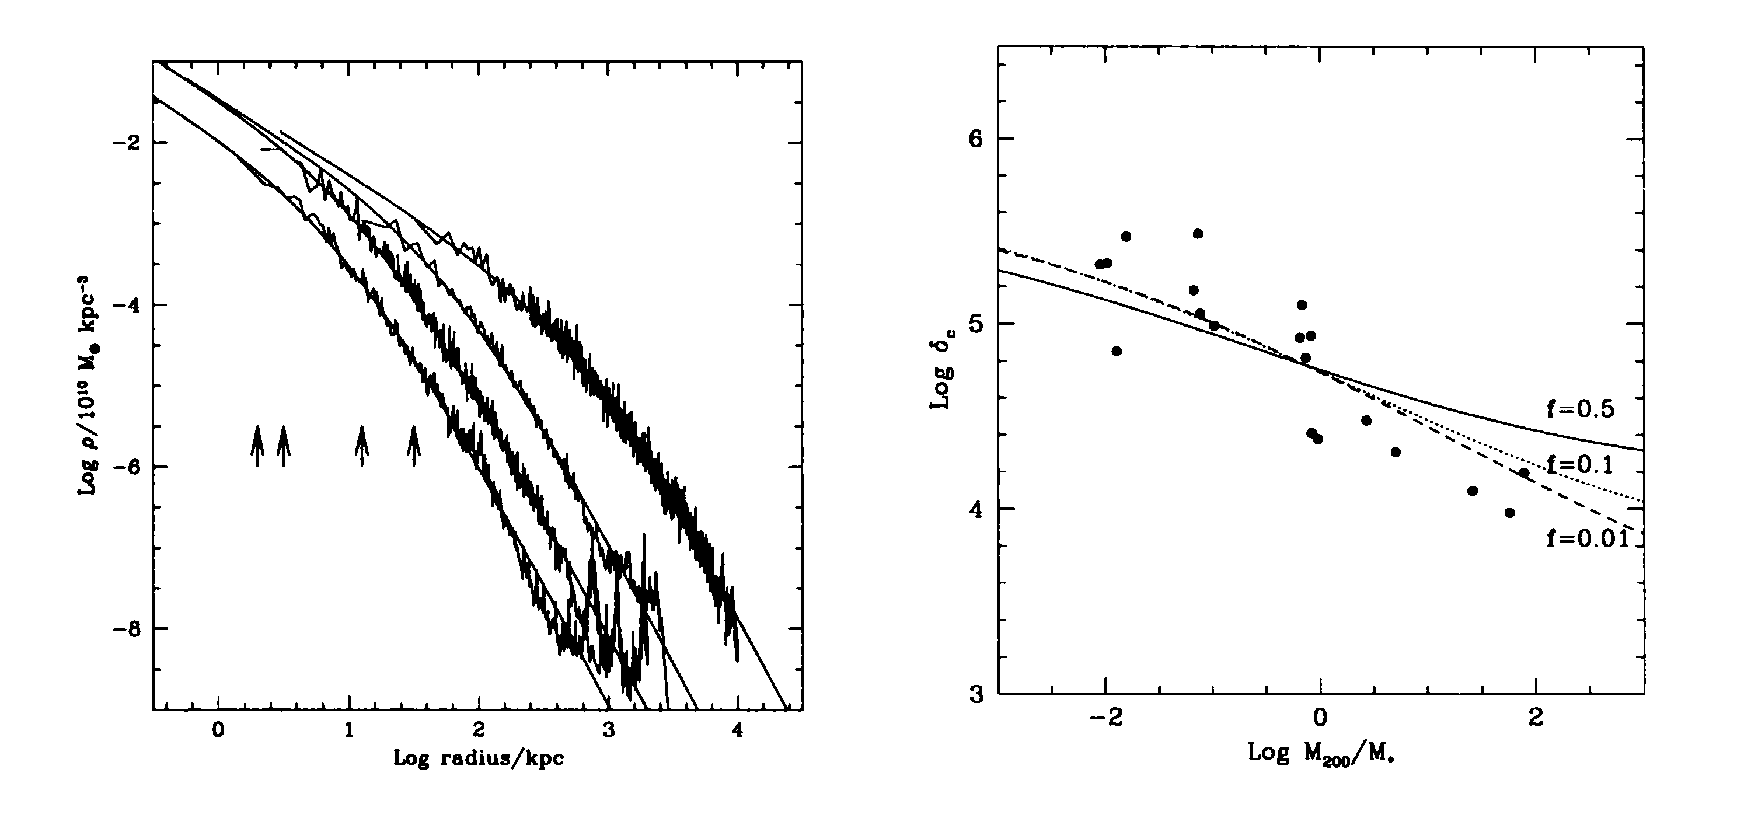
\includegraphics[width=0.77\textwidth]{Pictures/DMhalos.pdf}
  \caption{\textit{Left:} Typical density profiles from \gls{cdm} halos obtained from N-body simulations. \textit{Right:} Characteristic overdensity of halos as a function of mass. Masses are expressed in units of the current non linear mass corresponding to the standard biased \gls{cdm} spectrum $M_{*}=3.3 M_{\odot}$. Figures from \cite{navarro_1996}.}
    \label{fig:DMhalos}
\end{figure}

\subsubsection{Dwarf Spheroidal Galaxies and Dark Clumps}

Following the standard model of cosmology, N-body simulations of the evolution of \gls{cdm} since the Big Bang predicts a hierarchical structure formation where \gls{dm} clusters into subhalos which merge into higher structures. The final picture at galactic scales, are galaxies embedded in a big \gls{dm} halo, surrounded by a population of subhalos with mass inversely proportional to their number \cite{2008DMhalossubhalosDSphe}. Simulations like Via Lactea II predict that the Milky Way is surrounded by a large number of \gls{dm} subhalos ($\sim 50,000$). The heavier of these substructures are the so called \gls{dsphe}. They are very faint galaxies (in optical) orbiting the Milky Way. Many of the observed \gls{dsphe} are strongly \gls{dm} dominated, but have absent or very little star formation and no signal of ionized or neutral gas \cite{2007Dwarfs}. Smaller structures with no emission at all are known as Dark Clumps. \\
These kind of objects are a perfect target for \gls{dm} searches because no $\gamma$-ray signal is expected from them due to ordinary astrophysical processes. Any $\gamma$-ray detection would be an unequivocal signal of \gls{dm} annihilation. \\
The present generation of $\gamma$-ray experiments have widely studied these objects in the search for \gls{dm}, not yet being succesful at detection but setting very stringent upper limits on \gls{dm} models using data from many \glspl{dsphe} (\cite{2010DSpheFermi}, \cite{2014DSpheHESS},\cite{2018DSpheMAGIC}, \cite{2017DSpheVERITAS}, \cite{2019DSpheCombined}).
\begin{figure}
\centering
 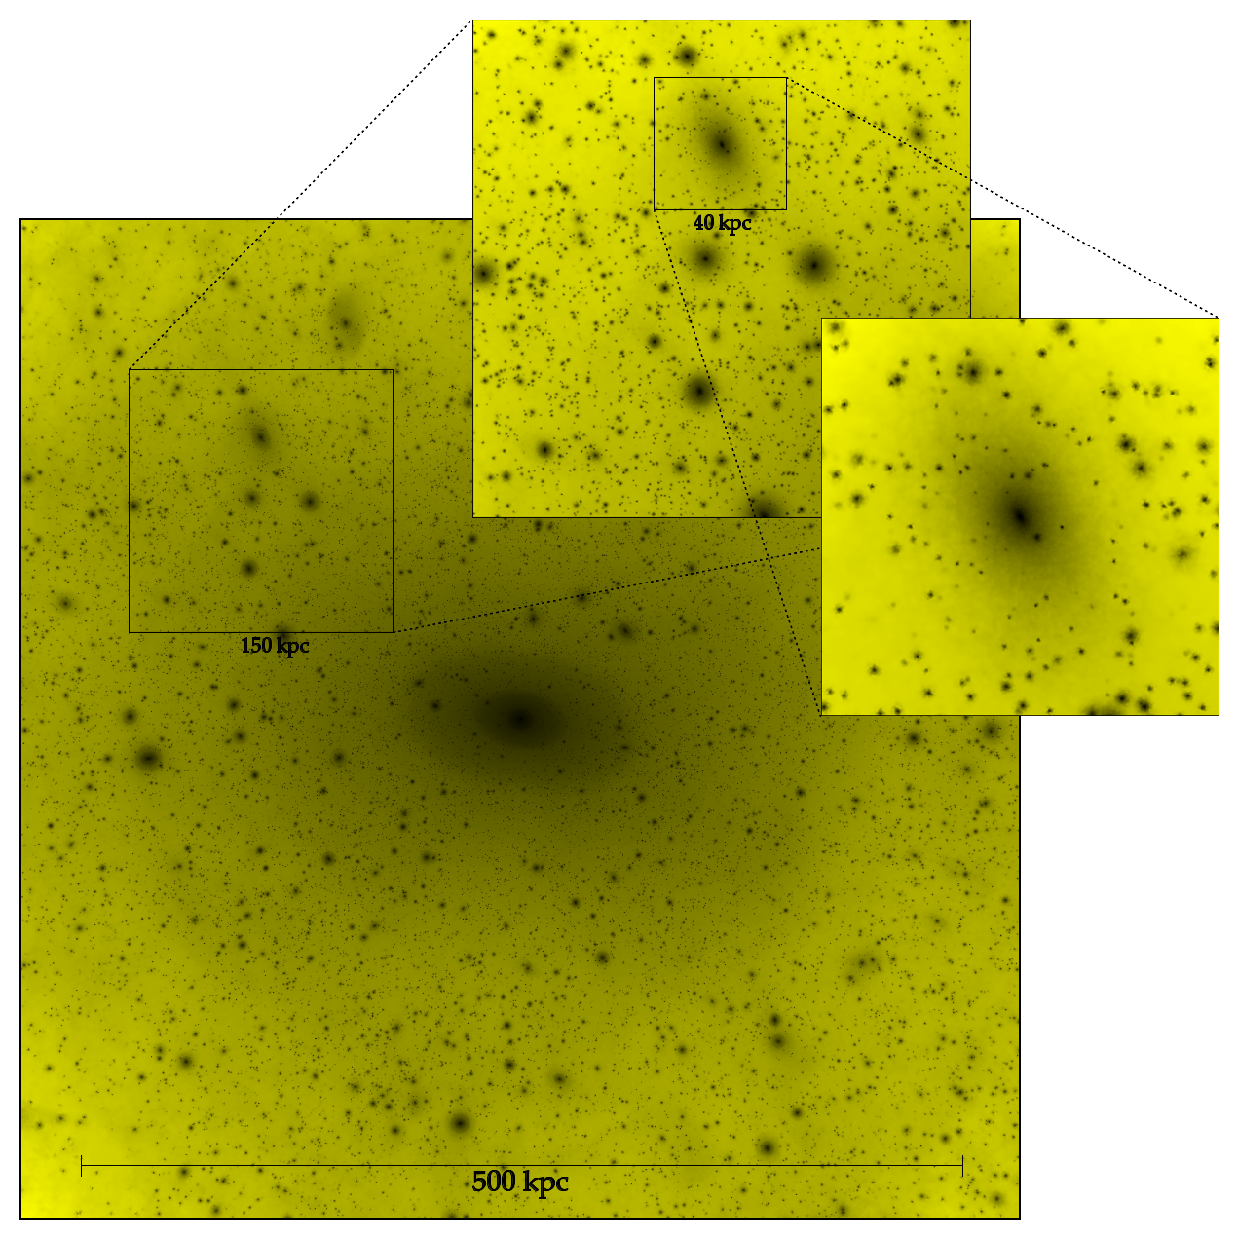
\includegraphics[width=0.77\textwidth]{Pictures/DMsubhalos.pdf}
  \caption{Results from \textit{Via Lactea} N-body simulations of \gls{dm} substructures. The picture show a projection of density squared in a 566 kpc $\times$ 566 kpc $\times$ 566 kpc region centered on the host halo at z = 0, from \cite{2008DMhalossubhalosDSphe}.}
    \label{fig:DMstructhalos}
\end{figure}

\subsubsection{Galaxy Clusters}

As has been mentioned before in section \ref{sec:clusters}, galaxy clusters are mostly dominated by \gls{dm} with a very high mass-to-light ratio. For this reason, they are good targets for indirect \gls{dm}  searches both for annihilation and decay. They are specially suitable for decaying \gls{dm}, since at large volumes the signal of decaying \gls{dm} which is proportional to the first power of the density overshines the signal of annihilation \cite{2012DecayingDMCirelli}.\\
Strong constraints for a wide number of models for \gls{dm} annihilation and decay have been set by \textit{Fermi}-LAT \cite{2012DMClustersDecayFermi}, \cite{2010DMClustersFermiAnnihilation} and \gls{hess} \cite{2012DMClustersHess}, and also constraints on the decaying lifetime of \gls{dm} were set by \gls{magic} \cite{2018DMClustersMAGIC}. 

\subsubsection{The Large Magellanic Cloud}

The \gls{lmc} has been considered a well promising target for \gls{dm} searches due to its proximity and rather high J-factor ($~10^{20} J/GeV^{2}cm^{-5}$). Kinematic studies of the \gls{lmc} show that more than half of the \gls{lmc} mass is forming a dark halo with a compact central bulge \cite{2006LMCkinematics}, \cite{1999LMCcentralbulge}.\\
\textit{Fermi}-LAT has used five years of data to set constraints on the \gls{dm} annihilation signal from the \gls{lmc} in the \gls{he} regime \cite{2015LMCDarkMatterFermi}. No limits has yet been set in the \gls{vhe} range though. 
As one of the main topics of this thesis, more on this subject will be extensively discussed in chapter ??.
\end{document}
